\chapter{General Method} \label{General Method}

\vspace*{-0.3cm}

The predictions developed in the previous chapter were investigated by conducting two studies: a corpus study and an experimental study. In each study the five affixes \prefix{un}, locative \prefix{in}, negative \prefix{in}, \prefix{dis} and \suffix{ly} were investigated. 
Since both studies were conducted to answer the same research questions, they were designed to be comparable.  

In both studies, multiple regression analysis was used to investigate which factors influence consonant duration with the five affixes under investigation. Multiple regression has the advantage of enabling us to look at the effect of one predictor in the presence of other, potentially intervening, predictors.  
To find out whether a word geminates, the influence of the number of consonants at the morphological boundary was investigated. In case of gemination, the double consonant (e.g. /nn/ in \textit{unnatural}) is longer than the correspondent singleton (e.g. /n/ in \textit{uneven}). In case of degemination, the double consonant is as long as the singleton. In addition to the number of consonants, I also tested the effects of other determinants of consonant duration and gemination. One the one hand, I tested the influence of phonetic, phonological and lexical factors which are assumed to affect duration, such as, for example, speech rate and stress. On the other, the investigated factors were chosen based on the predictions made in the last chapter. In other words, I tested the influence of factors which are predicted to affect consonant duration according to the different theories of the morpho-phonological interface discussed (cf. table \ref{tbl:Factors predicting gemination} in chapter \ref{Theory}). 




In the first part of this chapter, I will discuss general differences between corpus and experimental studies. This is important in order to understand why both types of studies were conducted. I will then describe the general methodology followed in both studies. After describing the composition of the data sets, I will explain the segmentation procedure of the sound files. Then, I will explain the main statistical models used in both studies. Finally, I will describe the variables included in the models.
Even though large parts of the methodology are the same in both studies, there are several aspects in which the studies' methodologies deviate from each other. The specific methodology for each study will be described in chapters \ref{Corpus Studies} and \ref{Experimental Studies}.\footnote{An earlier version of sections \ref{Acoustic Analysis}, \ref{stats}  and \ref{General method annotation} has been published in \cite{BenHedia.2017}.}


\section{Corpus Studies vs. Experimental Studies on Speech Production} \label{corpus and experimental studies}


% Corpus study: advantages
Corpus studies have the advantage of looking at natural conversational speech. As discussed by \cite{Tucker.2016}, it is of high importance to investigate this kind of speech in order to theoretically model speech production.  By reviewing previous studies \cite{Tucker.2016} demonstrate that conducting studies on carefully articulated speech does not suffice to shed light on speech production, and that there are profound differences between careful and conversational speech. The two types of speech deviate in word choice, sentence structure, tones and intonation, phonological assimilation and, crucially for this study, degree of speech reduction. Since degemination is realized by durational reduction of the double consonant, one can expect differences in gemination depending on the type of speech investigated. One would expect more reduction in natural conversational speech than in experimental careful speech. That the type of speech investigated is important for gemination is shown by the results in \cite{Oh.2012} where more reduction, i.e. a higher degree of degemination, was found in normal than in careful speech (see section \ref{previous empirical work} for discussion). One might therefore conclude that natural conversational speech, as found in a corpus, is better suited to investigate gemination in English than experimental careful speech.

% corpus studies: disadvantages
However, there are a number of drawbacks with investigating natural conversational speech. This type of speech is very hard to elicit in controlled experiments, and one therefore has to resort to corpora. As laid out by \citet[21]{Tucker.2016}, ``corpora come at a high cost in terms of their creation'', i.e. annotation and segmentation of the data is very time consuming. 
Furthermore, by their very nature corpus data entail various factors which are not controlled for, and which might confound results (such as contextual and pragmatic aspects of language). While a lot of these factors can be accounted for by using advanced statistical methods, corpus data will always be less controlled than experimental data, i.e. the potentially negative effect of confounding factors is always higher in corpus studies than in experimental studies (see also \citet[144]{Kunter.13.04.2017} for discussion).
An additional potential problem with corpus data is the number of types and tokens available in a given corpus. While for some phenomena a corpus might comprise a higher number of types and tokens than attainable in an experimental study, for other phenomena corpora may not feature higher numbers of types and tokens. This is the case with morphological gemination. As discussed in section \ref{scope of gemination}, morphological geminates are not frequent among prefixes. They do not occur very often in natural speech, and the corpus study in this work is restricted to a rather small set of types and tokens for some affixes. 

The small size of the data set entails an additional problem which is related to the composition of the data set. Since the choice of adequate items for the  corpus study is very limited, factors of interest are unevenly distributed among types in the study. Even though multiple regression models open up the opportunity to work with unevenly distributed data sets, some distributional aspects, such as the systematic co-occurrence of two or more factors, or the infrequency of types with specific attributes, cause problems which cannot be ignored.  They have to be taken into account when conducting statistical models, and when interpreting the results. Some potential effects on gemination might not be testable in the corpus study. Therefore, an experimental study needs to be conducted to complement the results of the corpus study.



% Experiment: great vareoty of types and tokens, everything under control BUT not natural

An experimental study has the advantage of offering the possibility to include a great variety of types and a high number of tokens. Furthermore, factors which possibly influence the duration of the boundary-adjacent consonant(s) can be controlled for in a carefully designed experiment. By choosing specific carrier sentences, as well as by a careful item selection, it is possible to control and manipulate factors, such as accentuation and word form frequency. 
However, experimental data are not as natural as corpus data and might therefore be argued to not represent natural speech processing. 

As one can see, the drawbacks of one type of study form the advantages of the other. While the corpus data provides natural conversational speech but only a small amount of viable types and tokens, the experimental data is less natural but enables one to more systematically investigate the factors of interest.
Following the approach taken by \cite{Arppe.2007} and \cite{Kunter.13.04.2017}, one can therefore state that the results of the corpus study and the ones from the experimental study complement each other to form a complete picture of the phenomenon under investigation, in this case the complete picture of the durational pattern of morphological geminates  for the five affixes \prefix{un}, locative \prefix{in}, negative \prefix{in}, \prefix{dis} and \suffix{ly}.
By conducting a corpus study and an experimental study I will furthermore be able to compare the results from spontaneous speech with the ones from experimental speech. This will give me the opportunity to detect differences in gemination depending on speech condition and affix. In other words, for each affix I will be able to find out which factors influence gemination at different levels of speech processing. As stated by \citet[1]{Arppe.2007}, ``each method adds to our understanding of the studied phenomenon, in a way which could not be achieved through any single method by itself''.




\section{Composition of the Data Sets} \label{General Method Data Sets}

To investigate gemination different structures were included in the data sets. The term \newterm{structure} refers to sets of words with a particular orthographic, phonological and morphological make-up. In this section, I will introduce the different structures included in the studies, and explain their relevance for the investigation.
 First, I will describe the structures investigated in the corpus study. Then, I will describe the structures investigated in the experimental study. Finally, I will give an overview of the composition of the data sets in both studies. The overview contains a comparison of the structures investigated in the corpus and the experimental study, as well as a summary of the type and token frequencies for both studies. A detailed description of how the items were selected in each study will be given in chapter \ref{Corpus Studies} and chapter \ref{Experimental Studies}.


\subsection{Corpus Study}\label{corpus data composition}
% 4 affixes in complex words

The tokens investigated in the corpus study were extracted from the Switchboard Corpus (\citealt{Godfrey.1997}), which consists of about 2400 two-sided phone conversations among North American speakers of English.  The data set was compiled of complex words featuring the five affixes \prefix{un}, locative \prefix{in}, negative \prefix{in}, \prefix{dis} and \suffix{ly}. As already discussed in section \ref{theory:in},  a word counted as morphologically complex if it showed the affixational meaning and if its base is attested outside the derivative with a similar meaning. It did not matter whether the base occurs as a free morpheme (e.g. \textit{natural} in \textit{unnatural}) or as a bound morpheme (e.g. \textit{-plicit} in \textit{implicit}  and  \textit{explicit}). 


% doubles as singles + im
To investigate whether the five affixes geminate it was essential to include two different structures. On the one hand, I included complex words which feature a phonological double consonant at the morphological boundary (e.g. \textit{unnatural}). On the other, I included complex words which feature a phonological singleton at the morphological boundary (e.g. \textit{uneven}). 
As discussed in section \ref{scope of gemination}, for the allomorph /ɪn/ morphological geminates are extremely rare. This is mirrored in the number of tokens of this category found in the Switchboard Corpus. It turned out that the corpus only contained 17 /ɪn/-prefixed tokens with a double /n/. There are only five different types with these tokens (\textit{innocuous, innovated, innovation, innovative, innovativeness}). Furthermore, out of these five types four share the same root. Because of the low frequency of double nasals with the allomorph /ɪn/, I decided to focus on the allomorph /ɪm/ instead, for which enough types exist. 
As discussed in section \ref{assumptions}, the literature very often is not explicit about the degemination behavior of the different allomorphs of \prefix{in}. If something is said, the authors state that all allomorphs behave in the same way, i.e. all allomorphs of \prefix{in} are taken to undergo degemination (e.g. \citealt{Borowsky.1986, Cruttenden.2014}). There is thus no obvious reason not to investigate the allomorph /ɪm/ as a representative of the morpheme \prefix{in}.  Investigating the allomorph /ɪm/ also has the advantage of giving us the possibility to directly link the results to the two previous studies on gemination which also analyzed /ɪm/ instead of /ɪn/. 

%Table + categores
Table \ref{tbl:overview structures environment corpus} gives an overview of  the structures investigated in the corpus study. The columns show the two structures which are essential to investigate gemination, i.e. phonological doubles in complex words and singletons in complex words. Examples for the different affixes are given in each line.\footnote{Note that both \prefix{in}prefixes, i.e. locative and negative \prefix{in}, were investigated in one data set. Therefore, they are not displayed separately at this point. The same holds for table \ref{tbl:overview structures environment experiment} and table \ref{tbl: Overview categories in each study}.} 
For singletons in complex words two different phonological environments exist, either the con-sonant-adjacent segment is a vowel or the consonant-adjacent segment is a consonant. Phonological doubles in complex words are always followed by a vowel. 



% Please add the following required packages to your document preamble:
% \usepackage{graphicx}
% \usepackage[table,xcdraw]{xcolor}
% If you use beamer only pass "xcolor=table" option, i.e. \documentclass[xcolor=table]{beamer}
\begin{table*}[]
	
	\caption{Overview of the investigated structures in the corpus study}
	\label{tbl:overview structures environment corpus}
	\centering
	%	\resizebox{\textwidth}{!}{%
	\begin{tabular}{cccc} \\
		%\multicolumn{3}{l}{\textbf{Durational difference}}
		& \begin{tabular}[c]{@{}c@{}}Phonological double\\ in complex word\end{tabular}                      & \multicolumn{2}{c}{\begin{tabular}[c]{@{}c@{}}Singleton\\ in complex word\end{tabular}}                         \\
		\hline
		\\
		\{un-\}  & 
		{ \begin{tabular}[c]{@{}c@{}}\color[HTML]{3166FF} \textit{unnatural}\\ (n\#nV)\end{tabular}}         & 
			{ \begin{tabular}[c]{@{}c@{}}\color[HTML]{3166FF} \textit{uneven}\\ (n\#V)\end{tabular}}         & 
			
					{ \begin{tabular}[c]{@{}c@{}}\color[HTML]{3166FF} \textit{untold}\\ (n\#C)\end{tabular}}         	               
		\\
		\\
		\{in-\}  & 
		
				{ \begin{tabular}[c]{@{}c@{}}\color[HTML]{3166FF} \textit{immortal}\\ (m\#mV)\end{tabular}}         & 
				 {NA}         & 
				
				{ \begin{tabular}[c]{@{}c@{}}\color[HTML]{3166FF} \textit{impossible}\\ (m\#C)\end{tabular}}         	\\
		
\\
		
		\{dis-\} & 
		{ \begin{tabular}[c]{@{}c@{}}\color[HTML]{3166FF} \textit{dissatisfy}\\ (s\#sV)\end{tabular}}         & 
		{ \begin{tabular}[c]{@{}c@{}}\color[HTML]{3166FF} \textit{disarm}\\ (s\#V)\end{tabular}}         & 
		
		{ \begin{tabular}[c]{@{}c@{}}\color[HTML]{3166FF} \textit{disgrace}\\ (s\#C)\end{tabular}}         	               
		\\
		\\
		
		\{-ly\}  & 
		{ \begin{tabular}[c]{@{}c@{}}\color[HTML]{3166FF} \textit{really}\\ (Vl\#l)\end{tabular}}         & 
		{ \begin{tabular}[c]{@{}c@{}}\color[HTML]{3166FF} \textit{truly}\\ (V\#l)\end{tabular}}         & 
		
		{ \begin{tabular}[c]{@{}c@{}}\color[HTML]{3166FF} \textit{probably}\\ (C\#l)\end{tabular}}         	               
		\\              
		\hline
	\end{tabular}%
	
	%	}

\end{table*}

%\newpage
%

Note that, throughout this book, I will use the term `environment' to refer to the particular combinations of phonological and morphological structure as found in the included types for each affix. In other words, the term `environment' refers to affix-specific combinations of sounds in a particular morphological structure.
The notation for the pertinent environments can be seen below each example. It is composed of the underlying consonant(s) in question and the neighboring segment (`V' for vowel, `C' for consonant). The `\#' marks a morphological boundary. These notations will be used in both studies throughout the book.


% only one 
For the prefix \prefix{in}, the table shows an empty slot for singletons in complex words with a following vowel. The reason is that there is no attested sequence /ɪmV/\todo{you sure about V?}, i.e. it is impossible to investigate /ɪm/-prefixed words with a following vowel. This is due to the allomorphy of the prefix. The prefix \prefix{in} only takes the form /ɪm/ when it is followed by homorganic consonants, i.e. by the bilabials /m/, /b/ or /p/. Thus, for /ɪm/-prefixed words containing a single nasal only the sequences /ɪmb/ and /ɪmp/ exist. 



\subsection{Experimental Study}\label{experiment data composition}

The tokens investigated in the experimental study were collected in two experiments conducted at the Cambridge University Phonetics Laboratory in October 2015 and October 2016. 
 As in the corpus study, complex words featuring the five affixes \prefix{un}, locative \prefix{in}, negative \prefix{in}, \prefix{dis} and \suffix{ly} were included  in the experimental study. One part of these words featured a phonological singleton at the morphological boundary, and one part  featured a phonological double at the morphological boundary. In addition to phonological doubles in complex words and singletons in complex words, two other structures were investigated in the experiment, orthographic doubles in simplex words and singletons in base words. The reason for not including these two structures in the corpus study is that not enough words with the pertinent structures were found in the Switchboard corpus. A statistical analysis of the tokens found in the corpus study was not reasonable.
 
 Table \ref{tbl:overview structures environment experiment} displays the four structures investigated in the experimental study. As in table \ref{tbl:overview structures environment corpus}, the columns of the table display the investigated structures, and examples of the structures are given in each line for each affix. The notation for the pertinent environment is given below each example. 
 
 

% Please add the following required packages to your document preamble:
% \usepackage{graphicx}
% \usepackage[table,xcdraw]{xcolor}
% If you use beamer only pass "xcolor=table" option, i.e. \documentclass[xcolor=table]{beamer}
\begin{table}[]
	
	\caption{Overview of the investigated structures in the experimental study}
	\label{tbl:overview structures environment experiment}
	\centering
	\resizebox{\textwidth}{!}{%
		\begin{tabular}{cccccc} \\
			& Phonological double             & Orthographic double & \multicolumn{2}{c}{Singleton }    & Singleton            \\
						&  in complex word                & in simplex word & \multicolumn{2}{c}{in complex words}    &  in base             \\
			
			\hline
			\\

		\{un-\}  & 
		{ \begin{tabular}[c]{@{}c@{}}\color[HTML]{3166FF} \textit{unnatural}\\ (n\#nV)\end{tabular}}         & 
		NA&
		{ \begin{tabular}[c]{@{}c@{}}\color[HTML]{3166FF} \textit{uneven}\\ (n\#V)\end{tabular}}         & 
		
		{ \begin{tabular}[c]{@{}c@{}}\color[HTML]{3166FF} \textit{untold}\\ (n\#C)\end{tabular}}      &
		   	    { \begin{tabular}[c]{@{}c@{}}\color[HTML]{3166FF} \textit{natural}\\ (\#n)\end{tabular}}               
		\\
		\\
			\{in-\}  & 
			{\begin{tabular}[c]{@{}c@{}}\color[HTML]{3166FF} \textit{immortal}\\ (m\#mV)\\ \color[HTML]{3166FF} \textit{innumerous}\\ (n\#nV)\end{tabular}} & NA                                                                            &
			
			 {\begin{tabular}[c]{@{}c@{}}NA \\ \phantom{more space } \\ \color[HTML]{3166FF} \textit{inefficient }\\ (n\#V)\end{tabular}} &
			 
			 {\begin{tabular}[c]{@{}c@{}}\color[HTML]{3166FF} \textit{impossible}\\  (m\#C)\\ \color[HTML]{3166FF} \textit{intolerant}\\  (n\#C)\end{tabular}} &
			
			 {\begin{tabular}[c]{@{}c@{}}\color[HTML]{3166FF} \textit{mortal}\\ (\#mV)\\ \color[HTML]{3166FF} \textit{numerous}\\ (\#nV)\end{tabular}} \\
			\\
			
			\{dis-\}  &
			{\begin{tabular}[c]{@{}c@{}}\color[HTML]{3166FF} \textit{dissatisfy}\\ (s\#sV)\end{tabular}}                      &
			{\begin{tabular}[c]{@{}c@{}}\color[HTML]{3166FF} \textit{dissertation}\\ (sV)\end{tabular}}          &
		{ \begin{tabular}[c]{@{}c@{}}\color[HTML]{3166FF} \textit{disarm}\\ (s\#V)\end{tabular}}         & 
		
		NA    	
			 & {\begin{tabular}[c]{@{}c@{}}\color[HTML]{3166FF} \textit{satisfy}\\ (\#sV)\end{tabular}}                   \\
			\\
			
			\{-ly\} &
			{\begin{tabular}[c]{@{}c@{}}\color[HTML]{3166FF} \textit{really}\\ (Vl\#l)\end{tabular}}                           & {\begin{tabular}[c]{@{}c@{}}\color[HTML]{3166FF} \textit{belly}\\ (Vl)\end{tabular}}                 & 
		{ \begin{tabular}[c]{@{}c@{}}\color[HTML]{3166FF} \textit{truly}\\ (V\#l)\end{tabular}}         & 
		
	NA    	         
			& {\begin{tabular}[c]{@{}c@{}}\color[HTML]{3166FF} \textit{real}\\ (Vl\#)\end{tabular}}                     
			
			\\	\hline
		\end{tabular}%
		
	}
	
	
\end{table}



I included orthographic doubles in simplex words, i.e. simplex words  which feature a similar phonological make-up as the investigated affixed words, and which are spelled with an orthographic double, to investigate possible effects of orthography on gemination.
That there is a relation between the orthography of a word and its phonology and phonetics is well established in the literature (see, for example, \citealt{Smith.1976,Ehri.1993,Warner.2004,Warner.2006,Brewer.2008,Berg.2016}). 
\cite{Brewer.2008}, for instance, found that the duration of a segment is influenced by the number of graphemes it is represented by. The more graphemes are present, the longer the duration of the segment becomes. Similarly,
\cite{Warner.2004} and \cite{Warner.2006} found an effect of orthography on duration in Dutch. In their data phonological singletons which are represented by orthographic doubles (e.g. /t/ in \textit{baatten}) are longer than phonological singletons which are represented by orthographic singletons (e.g. /t/ in \textit{baten}). \citeauthor{Warner.2004}'s results suggest that gemination might not be a morpho-phonological phenomenon but an orthographic one. In other words, there is the possibility that the lengthening of double consonants is merely an orthographic effect and not a morpho-phonological effect.
To test this possibility orthographic doubles in simplex words were included.
In contrast to phonological doubles in complex words, they only feature one underlying consonant (e.g. \textit{di}/ss/\textit{atisfy} vs. \textit{di}/s/\textit{ertation}). 
If  orthographic doubles in simplex words are longer than singletons in complex words, the number of underlying consonants is irrelevant for gemination.  In that case, gemination is an orthographic phenomenon. 
If, on the other hand, orthographic doubles in simplex words are as long as singletons, and if they are simultaneously shorter than  phonological doubles in complex words, gemination is a morpho-phonological phenomenon. In this case, only words with two underlying consonants geminate.

\clearpage

Simplex words with orthographic doubles that feature the same phonemic strings as the investigated affixes are extremely rare. The number of simplex words with an orthographic double starting in /ʌn/, /ɪn/ or /ɪm/ is so small that a statistical investigation is not reasonable. Only for words with the phonemic strings /dɪs/ and /li/ a sufficient number of types exists. Therefore, the effect of orthographic doubles was only investigated for /dɪs/ and /li/. 


% base words
The fourth structure investigated in the experimental study are phonological singletons in base words. I included the base words of all complex words with an underlying double consonant, e.g. \textit{natural} for \textit{unnatural} and \textit{real} for \textit{really}. For prefixes, the base words were included to compare the duration of the double consonant in the complex word with the base-initial consonant in the base word. For suffixed words the double consonant was compared to the base-final consonant, respectively. This comparison was conducted to ensure that the potential lengthening of the morphological geminate was not caused by an inherently long base-initial consonant (or base-final consonant in case of \suffix{ly}, respectively).


As can be seen in table \ref{tbl:overview structures environment experiment}, in addition to  the allomorph /ɪm/  the experimental study also investigated /ɪn/ to test gemination with \prefix{in}. This is different from the corpus study in which, due to a low token frequency of morphological geminates with /ɪn/, only /ɪm/ was investigated.  

For the affixes \prefix{dis} and \suffix{ly}, the phonological environment was kept constant across all structures. In all words, the consonant(s) of interest is adjacent to a vowel. 
The phonological environment was kept constant to avoid effects of the affix-adjacent segment on the duration of the consonant(s) of interest. Due to the limited choice of types and tokens in the corpus study, controlling the phonological environment across words was only possible in the experimental study.%, i.e. not in the corpus study.

It would have also been possible to keep the following segment constant across all words for the prefix \prefix{un} and the allomorph /ɪn/. However, for the allomorph /ɪm/ the phonological environment cannot be kept constant across structures. In case of a singleton at the morphological boundary, the allomorph is always followed  by a stop consonant, i.e. /p/.\footnote{Because of low type frequency of items with a following /b/, and to keep the environment as constant as possible, no \prefix{in}prefixed items with a following /b/ were included in the study.} Doubles are always followed by a vowel. This evokes the problem of the interpretation of potential durational differences between doubles and singletons for /ɪm/, i.e. it is unclear whether potential differences are caused by the number of consonants or the deviating phonological environment. Teasing apart the two effects is impossible for /ɪm/.

However, teasing apart the effect of the number of consonants from the effect of the following segment is possible for \prefix{un} and /ɪn/. As shown in table \ref{tbl:overview structures environment experiment}, for \prefix{un} and /ɪn/ the singleton environment with a following vowel (n\#V) exists and was included in the study. I also included the environment n\#C for /ɪn/ and \prefix{un}prefixed words in the data set.
 One can thus analyze durational differences in \prefix{un} and /ɪn/-prefixed words across the three environments  n\#nV, n\#V and n\#C. 
This makes it possible to see which durational differences can be expected between nasals with a deviating number of underlying consonants (durational difference between n\#nV and n\#V), and which durational differences can be expected between nasals with deviating following segments (durational difference between n\#V and n\#C). 
The differences in duration between the environments for \prefix{un} and /ɪn/ can then be used as a reference for the durational pattern of /ɪm/. 
In other words, one can compare the durational differences found for /ɪm/ with the ones found for \prefix{un} and /ɪn/.\footnote{Note that in all \prefix{un} and \prefix{in}prefixed words with an n\#C-environment, the following consonant is /t/ (e.g. \textit{untold, intolerant}). The consonant /t/ was chosen because of its comparability to /p/, i.e. the consonant following /ɪm/-prefixed words with a singleton. In both cases a stop which shares its place of articulation with the preceding nasal follows the prefix.}
In turn, one can find out whether the potential difference between singletons and doubles for /ɪm/ should be interpreted as gemination, or whether it is merely caused by differences in their phonological environments.

%\enlargethispage{2\baselineskip}




%\clearpage
\subsection{Overview of the Data Sets}

%The table
Table \ref{tbl: Overview categories in each study} gives an overview of the composition of the data sets in the two studies.
On the left side of the table the environments investigated in the corpus study are displayed, on the right the ones of the experimental study. 
For each affix (and in case of \prefix{in} its allomorphs), the included environments are indicated in the pertinent fields by the annotation introduced in table \ref{tbl:overview structures environment corpus}.
For example, the corpus study includes the following three environments for \prefix{un}prefixed words: phonological double nasals in complex words followed by a vowel (n\#nV), singleton nasals in complex words followed by a vowel (n\#V) and singleton nasals in complex words followed by a consonant (n\#C). In the middle column of the table examples for each environment are given.

%\enlargethispage{-2\baselineskip}
% 9 data sets because of inherent durational differences between the
For the analysis, I generated subsets for each affix (and in case of \prefix{in} its allomorphs). This was necessary because the duration of a consonant heavily depends on its type. For example, fricatives are generally longer than nasals, and nasals are generally longer than laterals (see, for example,  \citealt{Umeda.1977}). For the affixes investigated in this study this means that out of the affixational consonants investigated the fricative in \prefix{dis}prefixed words will most likely be the longest, followed by the nasals in \prefix{un} and \prefix{in}prefixed words. The /l/ in \suffix{ly}-suffixed words is expected to be the shortest. Even within types of consonants there are major differences 
in duration. \cite{Umeda.1977}, for instance, found that bilabial nasals in word-medial position are almost twice as long as alveolar nasals in the same position (74 ms vs. 38 ms). 
Affixes which differ in their phonological make-up must therefore be investigated separately with regard to their duration, i.e. it is necessary to analyze the duration of the different consonants in different analyses. % As can be seen in table \ref{tbl: Overview categories in each study}, this lead to the creation of four subsets in the corpus study. For the experimental study five subsets were generated.



% \usepackage[table,xcdraw]{xcolor}
% If you use beamer only pass "xcolor=table" option, i.e. \documentclass[xcolor=table]{beamer}
\begin{table*}[t!]
	\caption{Overview of subsets and investigated environments in the two studies}
	\label{tbl: Overview categories in each study}
	\centering
	\begin{tabular}{lccc}
		\\
		& \textbf{Corpus Study }                                                                                                                                                                               & \textbf{Example}                                                                                                                                             & \textbf{Experimental Study}                                                                                                        \\ \hline
		
		un- & {\color[HTML]{000000} \begin{tabular}[c]{@{}c@{}}n\#nV \\ n\#V \\  n\#C\\ \phantom{CV}\end{tabular}}                                                                              & {\color[HTML]{3166FF} \textit{\begin{tabular}[c]{@{}c@{}}unnatural\\ uneven\\ untold\\ natural\end{tabular}}}                                                & {\color[HTML]{000000} \begin{tabular}[c]{@{}c@{}}n\#nV\\ n\#V \\  n\#C\\ \#nV\end{tabular}}
			\\ \hline
		
		in-  & & {\color[HTML]{3166FF} \textit{\begin{tabular}[c]{@{}c@{}}innumerous\\ inefficient\\ intolerant\\ numerous\end{tabular}}} & {\color[HTML]{000000} \begin{tabular}[c]{@{}c@{}} n\#nV\\  n\#V\\  n\#C\\ \#nV\end{tabular}}   \\ \hline
		
		
		im-  & {\color[HTML]{000000} \begin{tabular}[c]{@{}c@{}}m\#mV\\ m\#C\\ \phantom{CV} \end{tabular}} & {\color[HTML]{3166FF} \textit{\begin{tabular}[c]{@{}c@{}}immortal\\ impossible\\ mortal\end{tabular}}} & {\color[HTML]{000000} \begin{tabular}[c]{@{}c@{}}m\#mV\\ m\#C\\ \#mV \end{tabular}}   \\ \hline
		
		dis- & {\color[HTML]{000000} \begin{tabular}[c]{@{}c@{}}s\#sV\\ s\#V\\ s\#C\\ \phantom{CV} \\ \phantom{CV}\end{tabular}}                                                               & {\color[HTML]{3166FF} \textit{\begin{tabular}[c]{@{}c@{}}dissatisfy\\ disarm\\ disgrace\\ satisfy\\ dissertation\end{tabular}}}                        & {\color[HTML]{000000} \begin{tabular}[c]{@{}c@{}}s\#sV\\ s\#V\\ \\ \#sV\\ ssV\end{tabular}}                          \\ \hline
		
		-ly  & {\color[HTML]{000000} \begin{tabular}[c]{@{}c@{}}Vl\#l\\ C\#l\\ V\#l\\ \phantom{CV}\\  \phantom{CV}\end{tabular}}                                                              & {\color[HTML]{3166FF} \textit{\begin{tabular}[c]{@{}c@{}}really\\ probably\\ truly\\ real\\ belly\end{tabular}}}                                     & {\color[HTML]{000000} \begin{tabular}[c]{@{}c@{}}Vl\#l\\ \\  V\#l\\ Vl\#\\ Vll\end{tabular}}                        \\ \hline 
	\end{tabular}
\vspace*{-0.3cm}
	
\end{table*}




Table \ref{tbl:token distribution both studies} gives an overview of the type and token distribution in each study. For each subset, the number of investigated types and tokens is given in the table.\footnote{Note that locative and negative \prefix{in} have the same phonemic form, and that they can therefore be analyzed in one data set.} The compilation of the data sets will be discussed in detail in chapters \ref{Corpus Studies} and \ref{Experimental Studies}.


\begin{table*}[h!]
	\caption{Type and token distribution across subsets in the two studies}
	\label{tbl:token distribution both studies}
	\begin{center}
		  	%	  			\renewcommand{\arraystretch}{1.3}
		\begin{tabular}{lrrrrr}
			
		&	\multicolumn{2}{r}{\textbf{Corpus Study} } &\multicolumn{2}{r}{\textbf{Experimental Study}} \vspace*{0.3cm}
		\\ 

			& Types & Tokens & \hspace*{3cm} Types & Tokens \\
			\hline
			{un-} \hspace*{1cm} & 101&158 &89 & 2615\\
			{in-}&&& 83 & 1232\\ 
			{im-}& 83 & 156 &  64&  1635\\ 
			{dis-} &64& 128 &59&1114  \\ 
			{-ly}& 150&  154 & 103& 1645 \\ 
			\hline
			Total & 398 & 596& 398& 8241\\
			
			\hline


		\end{tabular}
	\end{center}
\end{table*}







%\newpage


\section{Acoustic Analyses}\label{Acoustic Analysis}
%\enlargethispage{\baselineskip}
After all sound files were extracted from the corpus and the experimental recordings, the data was segmented and phonetically transcribed using the software Praat (\citealt{Boersma.2014}). For each token, the segments of the affix in question, as well as the segments of the syllable immediately following or preceding the affix under investigation, were annotated. Figure \ref{fig:segmentation unneeded} displays an example. As can be seen in the figure, doubles were segmented as one segment. This is because in almost all cases no boundary between the two adjacent consonants was distinguishable. Only for some words in the experimental data a pause was uttered between the affix and the base, i.e. the two consonants were pronounced as two independent segments. These tokens were noted down and will be discussed in chapter \ref{Experimental Studies}.

\begin{figure*}[]
	\centering
	\fbox{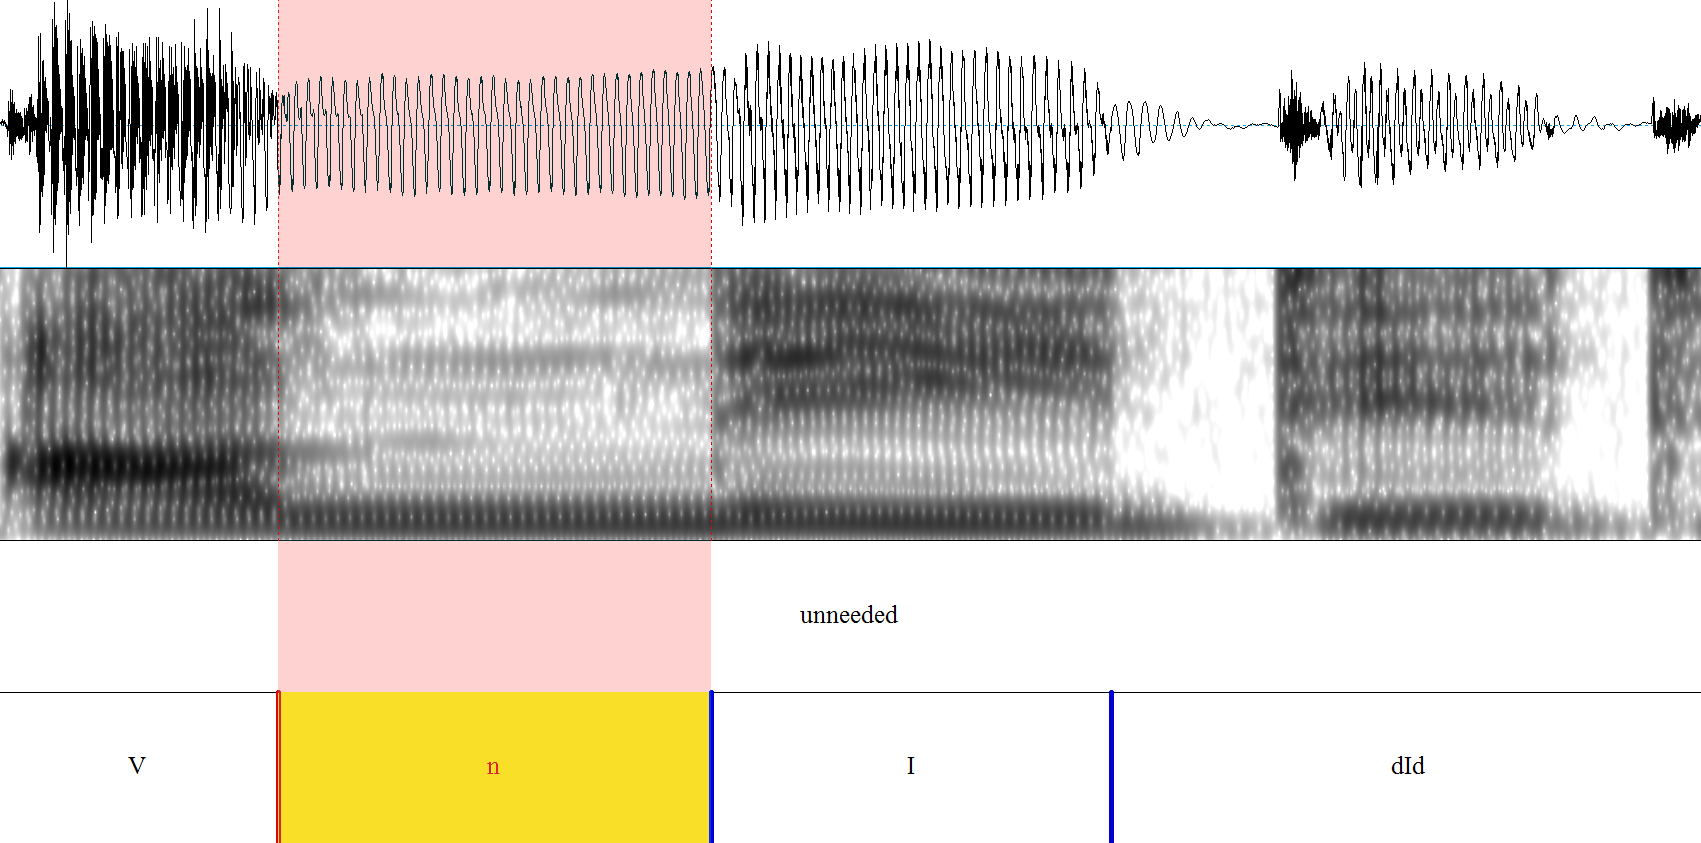
\includegraphics[width=11.5cm ,keepaspectratio]{images/GeneralMethod/segmentationUnneeded.png}}
	\caption{Segmentation example \textit{unneeded}}
	\label{fig:segmentation unneeded}
\end{figure*}

There are two possible ways of segmenting speech data, manual segmentation and automatic segmentation. Automatic segmentation has the major advantage of demanding a lower workload and less time than manual segmentation. Furthermore, one can expect automatic segmentation to be very systematic. This is because automatic segmentation relies on forced aligners which are based on algorithms. These algorithms ensure that every file is segmented according to the same criteria. This means, in contrast to manual segmentation, there is no risk of inter-annotator differences.

However, there are also major disadvantages with automatic segmentation. The forced aligners used in automatic segmentation rely on canonical pronunciations. This means that the forced aligner will always annotate all phonemes represented in the canonical pronunciation of a word, irrespective of whether they were produced by the speaker or not.  Especially in conversational speech words are sometimes drastically reduced, i.e not all sounds of a word are produced. This poses a serious problem for automatic segmentation. Segments which are not present are annotated by the system.
An additional problem is related to the fact that forced aligners do not analyze the whole sound file but instead analyze the file in increments of a few milliseconds. The forced aligner software WebMAUS (\citealt{Schiel.1999,Kisler.2016}), for instance, uses 10 ms increments. Especially when investigating fine phonetic detail these increments are problematic. For example, the duration of a word-medial /l/ is 40 ms on average (cf. \citealt{Umeda.1977}). Increments of 10 ms might distort the phonetic investigation of the duration of /l/ immensely by positioning a boundary 10 ms too early, or 10 ms too late, i.e. the automatic segmentation might show /l/ to be up to 50\% shorter or longer than it actually is.

To test the accuracy of automatic segmentation, i.e. to test whether automatic segmentation can be used in this study, I carried out an automatic segmentation on a subset of the corpus and the experimental data. I used the software WebMAUS (\citealt{Schiel.1999,Kisler.2016}) for the segmentation.  WebMAUS takes speech files with orthographic transcriptions as an input and gives segmented, phonologically transcribed text grids as an output. The segmentation is based on a production system, which takes the canonical pronunciations of an utterance, as well as its sound wave, and then, on the basis of a Viterbi alignment procedure, computes the most probable pronunciation variant. Based on this pronunciation variant the speech wave is segmented in 10 ms increments. 
 \clearpage
 
 The automatic segmentation of the subset showed that the automatic segmentation is inaccurate and therefore not suited to investigate fine phonetic detail. As expected, the system annotated sounds which were not present in the acoustic signal and misplaced boundaries, i.e. boundaries were set too early or too late in the speech signal. Especially for the corpus data the boundaries were very poorly placed. This might be due to the extreme reduction found in conversational speech. 
 Having a valid, reliable and precise segmentation is extremely important for this investigation. Therefore, it was decided to not use automatic segmentation but instead segment all sound files manually. I decided to not first use automatic segmentation and then adapt the set boundaries since revising the automatic segmentation holds the risk of influencing the annotator unconsciously. 
 

In contrast to automatic segmentation, manual segmentation is less prone to systematic mistakes and inaccuracies. This is because it does not rely on canonical representations and incremental analyses. It thus allows for more precise annotations than automatic segmentation.  However, there are also disadvantages with manual segmentation. 
First, it is very time-consuming. Second, it is prone to inconsistent, unsystematic boundary setting, as well as to inter-annotator differences. While the possibilities to speed up manual segmentation are very limited, there are various possibilities to prevent inconsistencies and inter-annotator differences. To ensure the reliability and validity of the manual segmentation, I applied the following four strategies: 1.  the development of strict segmentation criteria based on the specifics of each sound, 2.  intensive training of the annotators, 3. segmenting a proportion of the data twice, and 4. testing the influence of the annotator on the segmentation statistically. In the following I will discuss each strategy in detail.\\


\textbf{1. The development of strict segmentation criteria}\\

The criteria on which the segmentation was based were developed by consulting  the relevant phonetic literature (cf. \citealt{Ladefoged.1996,Johnson.1997b,Ladefoged.2003,Machac.2009,Ladefoged.2011}) and were optimized during the segmentation process. The final criteria will be described in the following. First, I will describe the criteria for the segmentation of the nasals in \prefix{un} and \prefix{in}words. Then, I will give a description of the criteria for fricatives in \prefix{dis}words. Finally, the criteria for laterals in \suffix{ly}-words will be given.\\

\clearpage

\textbf{The nasals in \prefix{un} and \prefix{in}prefixed words}\\

Nasals have a regular waveform which has a lower amplitude than the waveform of vowels. Formants of nasals are quite low and faint in comparison to those of vowels. Boundaries between the preceding vowel and the nasal were thus set where the acoustic energy drops in the waveform, the spectrogram becomes visbily fainter and the higher formants visibly decrease (see figure \ref{fig:segmentation unneeded}). In case of a following vowel, the boundary was marked at the point where the amplitude increases in the waveform and the formants become clearly visible (see figure \ref{fig:segmentation unneeded}).  Since approximants have, similar to vowels,  a higher amplitude than nasals, as well as more acoustic energy, the identification of approximants following the nasal was similar to the identification of a following vowel. If a stop followed the nasal, the boundary was marked at the beginning of the occlusion, which was identified by the abrupt decrease of the waveform and the sudden diminishment of the formants (see figure \ref{fig:segmentation imprint}). In case of a following fricative, the boundary was set where the waveform became visibly irregular and the energy was concentrated in the upper part of the spectrogram with no distinct formants visible. All boundaries were set at the nearest zero crossing of the waveform.\\

%\newpage
% additional figure for in+V

%\begin{figure}[h!]
%	\centering
%	\fbox{\includegraphics[width=\textwidth,height=\textheight,keepaspectratio]{"images/General Method/segmentation inobservable"}}
%	\caption{example segmentation inobservable}
%	\label{fig:segmentation inobservable}
%\end{figure}

\begin{figure}[h!]
	\centering
	%	\vspace{-0.2cm}
	\fbox{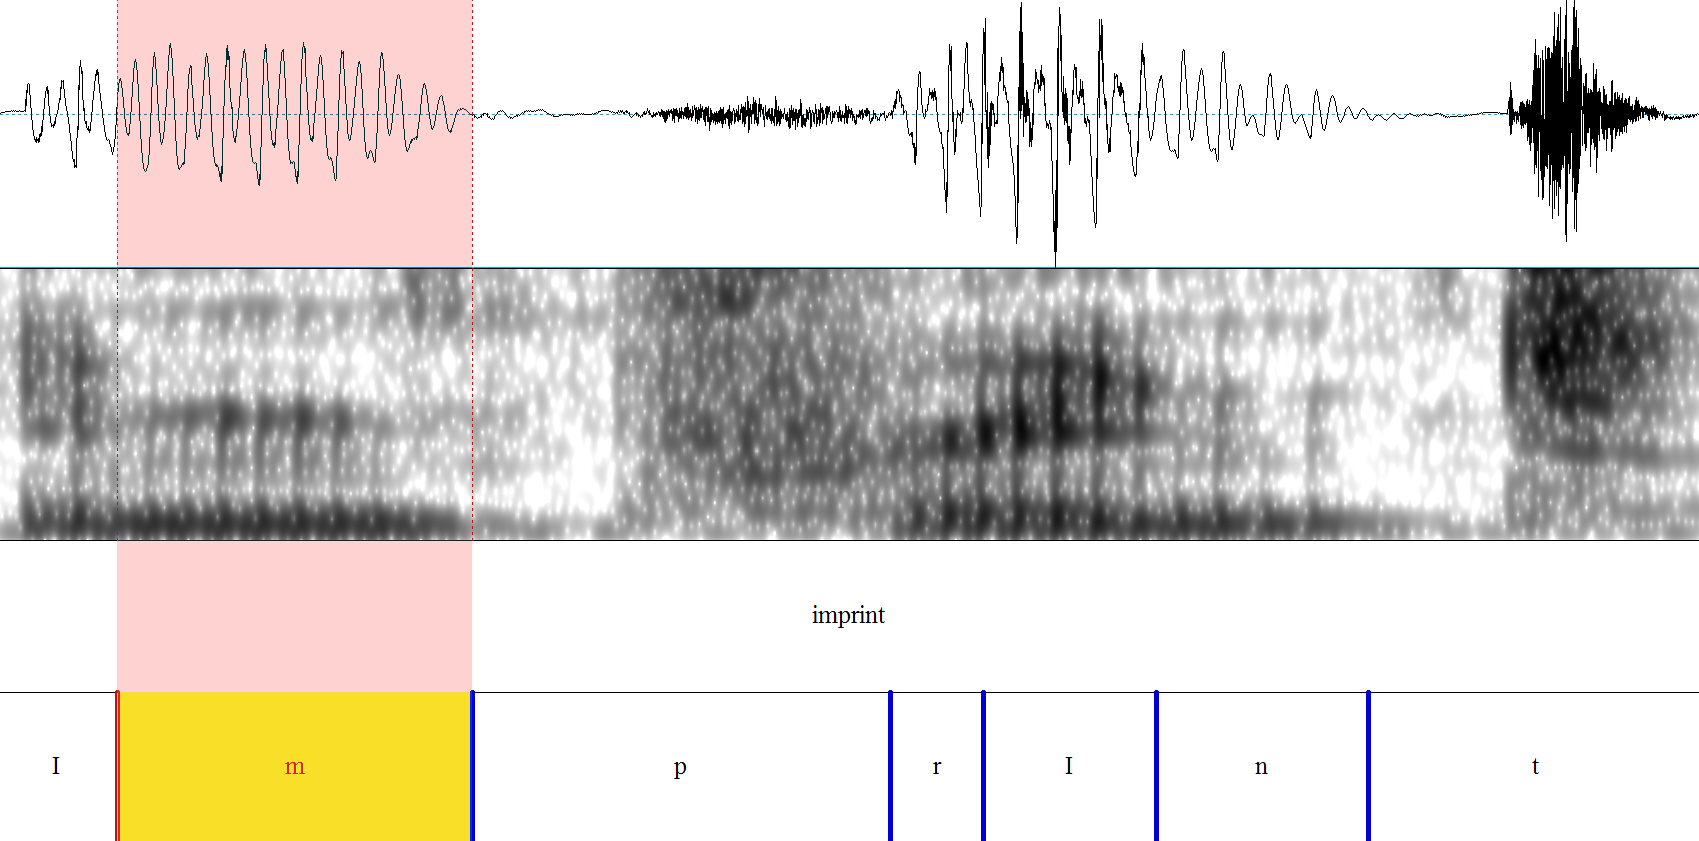
\includegraphics[width=11.5 cm ,keepaspectratio]{images/GeneralMethod/segmentationImprint.png}}
	\caption{Segmentation example \textit{imprint}}
	\label{fig:segmentation imprint}
%	\vspace{-0.5cm}
\end{figure}


\textbf{The fricative in \prefix{dis}prefixed words}\\




Fricatives are characterized by an irregular waveform, which is very easy to distinguish from the regular waveform of vowels. Furthermore, for fricatives, there is energy throughout the whole spectrogram and no separate formant bands are visible. Most energy is visible in the upper part of the spectrogram (see figure \ref{fig:segmentation dissident}). This is even more pronounced for voiceless fricatives, which are found in the majority of the \prefix{dis}prefixed words.
The boundary between the preceding vowel and the fricative was set where the waveform became irregular and the distinct formant structure vanished. The boundary between /s/ and the following vowel was set where the opposite was the case (see figure \ref{fig:segmentation dissident}). In case of a following approximant the same criteria were applied. If a stop followed the fricative, the boundary was marked at the beginning of the occlusion. There were no fricatives immediately following the prefixal /s/ in the data sets.\\

\begin{figure} [H]
	\centering
	\fbox{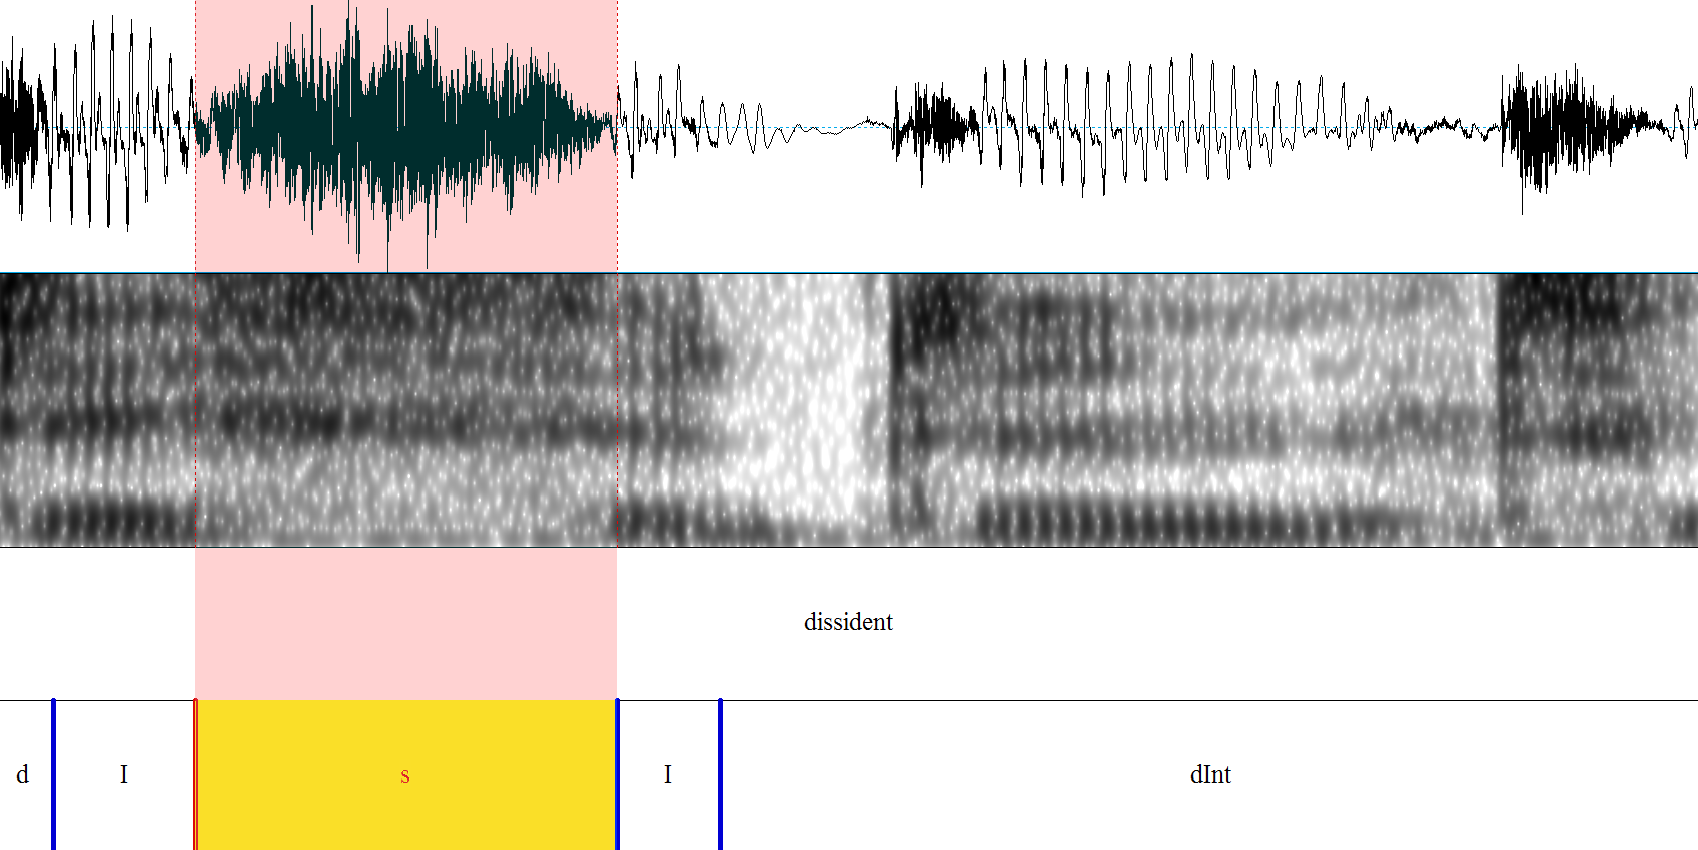
\includegraphics[width=11.5 cm ,keepaspectratio]{images/GeneralMethod/segmentationDissident.png}}
	\caption{Segmentation example \textit{dissident}}
	\label{fig:segmentation dissident}
\end{figure}



\textbf {The lateral in \suffix{ly}-suffixed words} \label{ly-segmentation}\\



% Most difficult segment to segment in data set --> a ot of exlcusion

Out of the four consonants investigated in this study, laterals are the most difficult to segment. This is due to the fact that laterals are very similar to vowels regarding their acoustical properties. Thus, it is quite challenging to set a boundary between vowels and laterals (see also \citet[chapter 7]{Machac.2009} for discussion). However, there are some aspects in which /l/ can be distinguished from vowels. There is less amplitude in the waveforms of laterals than in the one of vowels.  Furthermore, their formant structure is, in contrast to the one of vowels, constant and, due to less energy in the speech signal, the formants of /l/ are in general fainter than the ones of vowels. This is especially the case for higher formants. Since in the suffix -\textit{ly} the lateral is followed by a high vowel, which displays very much energy in the upper formants, it is possible to see the formant structure change between /l/ and the following vowel in my data sets. The boundary between /l/ and /i/ was thus set at the point at which the formant structure changed, i.e. the higher formants became more pronounced (see figure \ref{fig:segmentation solely}). For intervocalic /l/ a visible decrease in the waveform, as well as the change in formant structure was used to mark the beginning of /l/ (see figure \ref{fig:segmentation solely}).
 
\begin{figure*} [h!]
	\centering
	\fbox{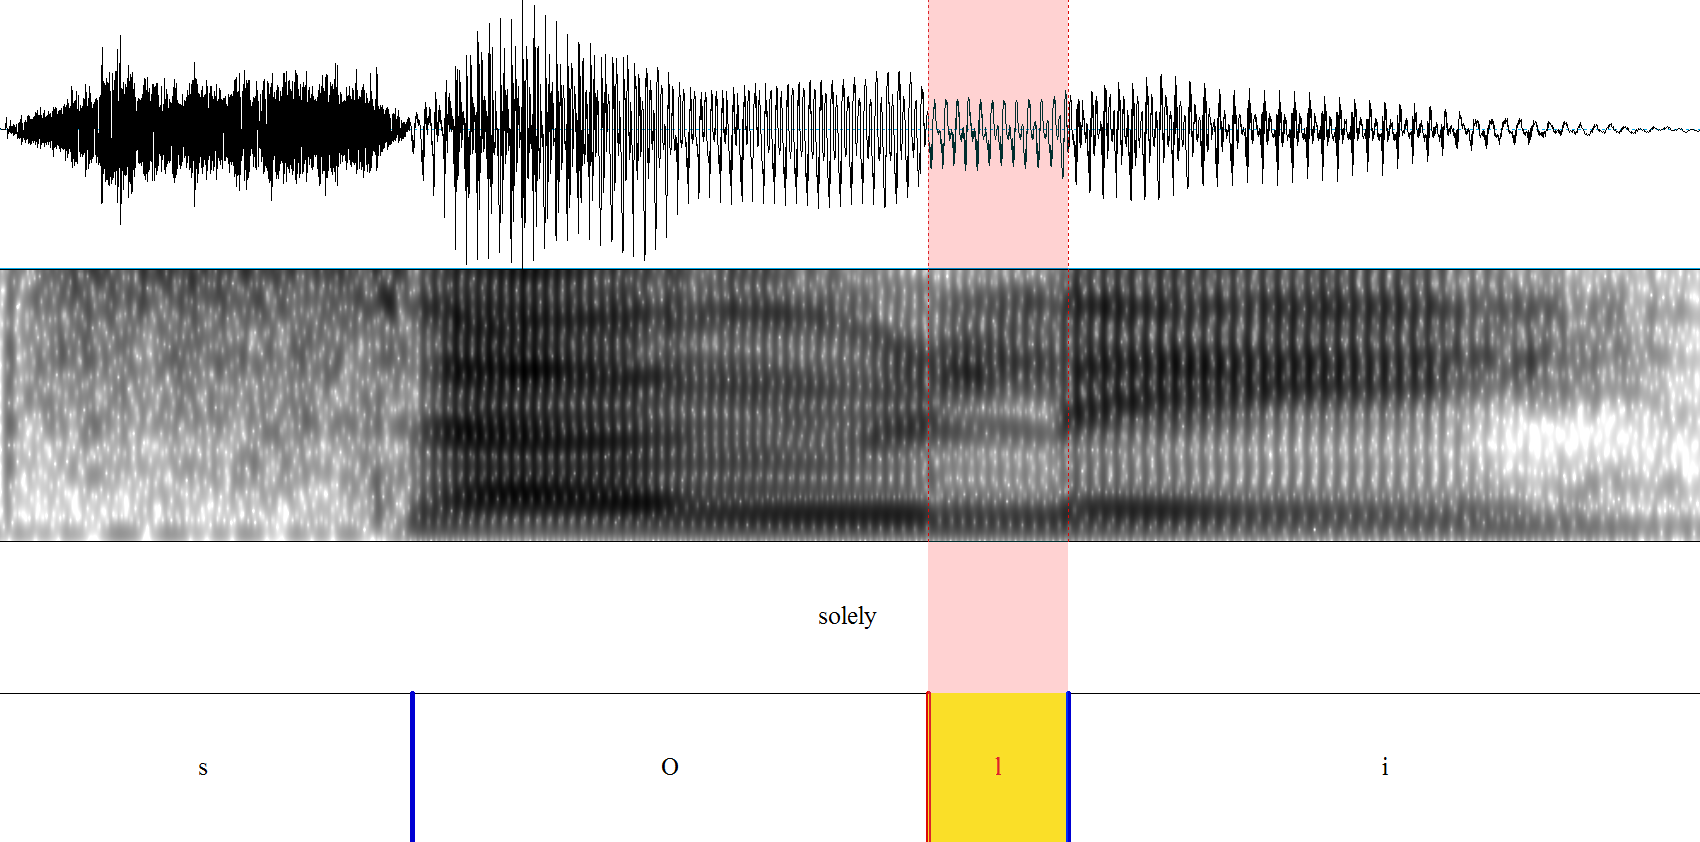
\includegraphics[width=11.5 cm ,keepaspectratio]{images/GeneralMethod/segmentationSolely.png}}
	\caption{Segmentation example \textit{solely}}
	\label{fig:segmentation solely}
\end{figure*}


Setting the boundaries between /l/ and a preceding consonant was generally not problematic since approximants can be distinguished quite easily from nasals, stops and fricatives. Approximants generally have a  higher amplitude and more energy in the spectrogram than nasals. Their waveform is periodic, whereas the waveform of fricatives, as well as the waveform of the aspirational phase of stops, is irregular.



\begin{figure*} [t!]
	\centering
	\fbox{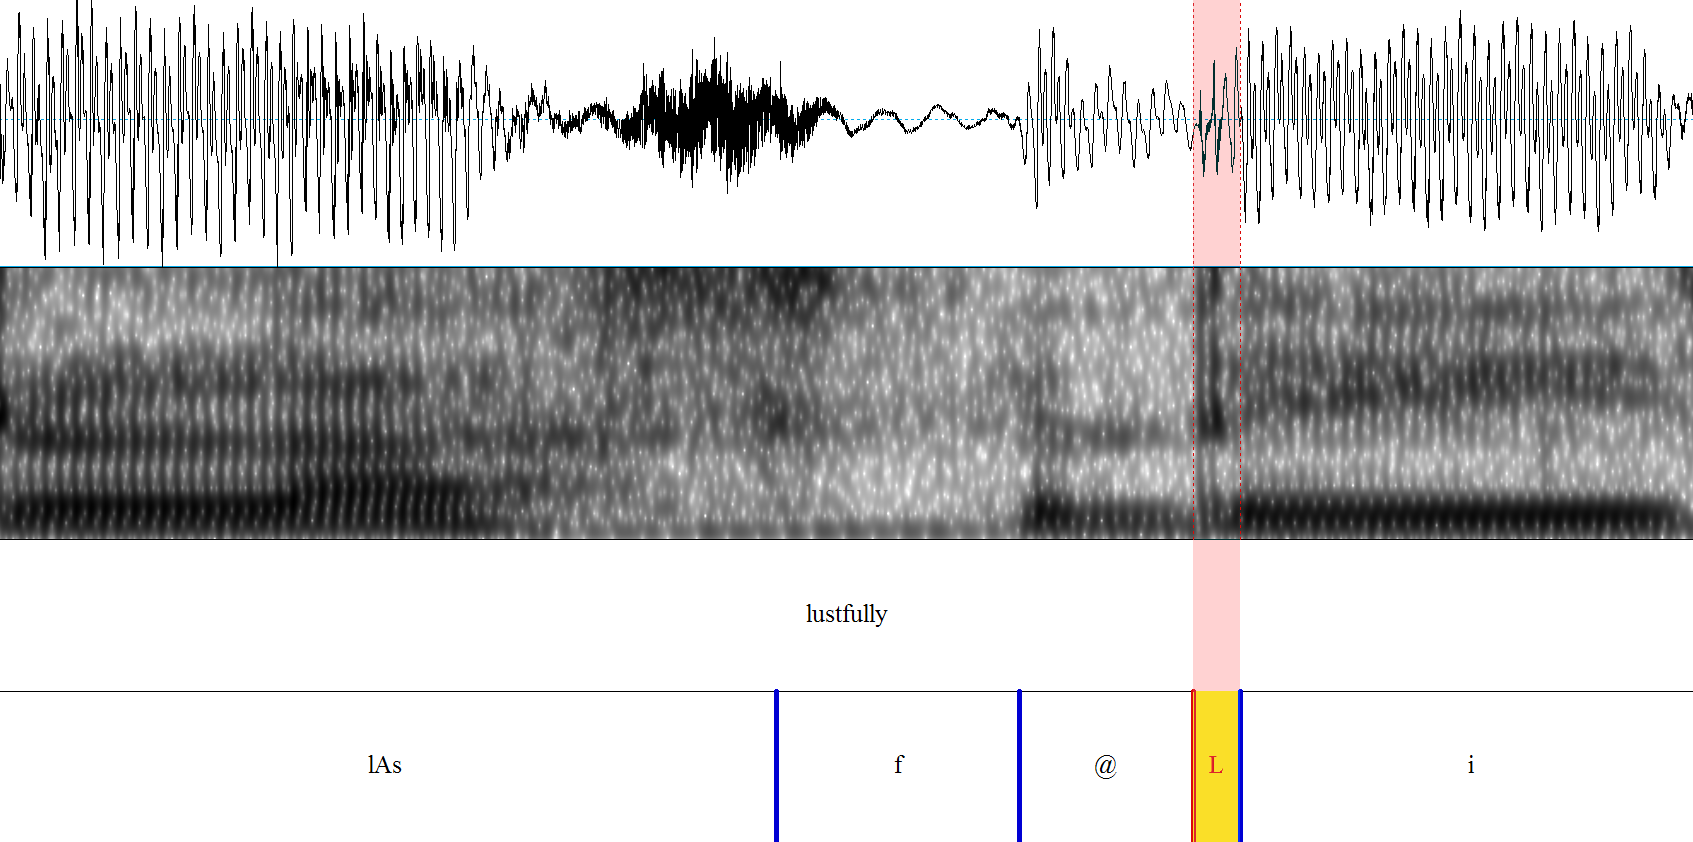
\includegraphics[width=11.5 cm ,keepaspectratio]{images/GeneralMethod/segmentationLustfully.png}}
	\caption{Segmentation example \textit{lustfully}}
	\label{fig:segmentation lustfully}
\end{figure*}


%\enlargethispage{1\baselineskip}
In some cases the waveform and the spectrogram for /l/ showed a completely different pattern. Figure \ref{fig:segmentation lustfully} shows a case in which /l/ is marked by a dark, vertical bar which stretches throughout the whole spectrogram. In this case /l/ is realized as a tap, i.e. not as an approximant. The bar marks the tongue release from the alveolar ridge. Because of the high amount of energy in the spectrogram /l/ can be easily set apart  from the neighboring vowels. This type of /l/ , i.e. a tap /l/, is generally shorter than the one described above, i.e. the approximant /l/. To account for this difference in duration the type of /l/ pronounced was coded in the variable \textsc{TypeOfL}. The variable was then incorporated in the statistical models as a covariate.\\

% very problematic at end of word - base words, often allomorphy, sometimes not visible at all



\begin{figure*} [b!]
	\centering
	\fbox{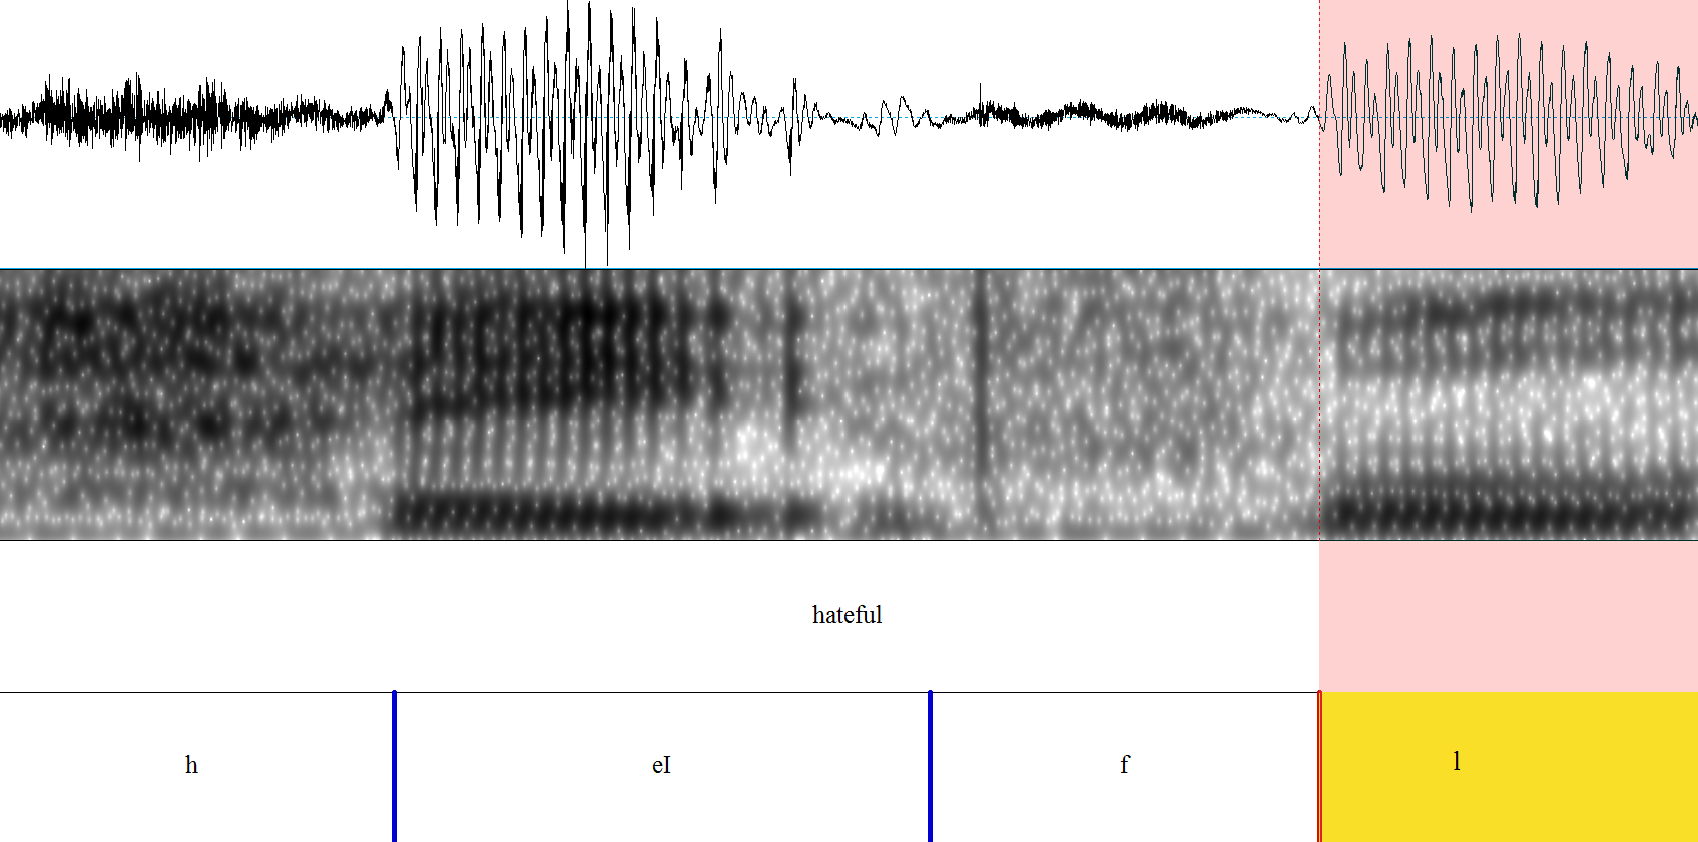
\includegraphics[width=11.5 cm ,keepaspectratio]{images/GeneralMethod/segmentationHateful2.png}}
	\caption{Segmentation example \textit{hateful}}
	\label{fig:segmentation hateful}
\end{figure*}

The criteria described above allowed for a valid and reliable segmentation of /l/. However, there were still items which were very difficult to segment. This was especially the case for items of the category l\#, i.e. /l/ at the end of base words (e.g. \textit{hateful, cool}). An example is displayed in figure \ref{fig:segmentation hateful}. There is no visible boundary between the preceding vowel and the lateral, i.e. the speaker did not pronounce them as two distinct sounds. There are various possible explanations, such as that the speaker might have deleted the word-final /l/, or that he might have vocalized it  while deleting the preceding vowel. Either way,  it is impossible to set a valid boundary between /l/ and the preceding vowel. Therefore, we marked the whole interval as /l/ (see figure \ref{fig:segmentation hateful}) and coded the pertinent tokens as featuring a vocalized /l/. Hence, the data set comprised three different types of /l/: the approximant /l/, the tap /l/ and the vocalized /l/. These three different types were coded in the variable \textsc{TypeOfL} with the values \texttt{approximant}, \texttt{tap} and \texttt{vocalized}.\\



\textbf{ 2.  Intensive training of the annotators}\\
% training

The corpus data was segmented by five annotators. The experimental data was segmented by six. The reliability of the segmentation criteria was verified by a set of trial segmentations.  In these trials the annotators segmented the same 30 items. If boundaries differed by more than 10 milliseconds, the annotators discussed the discrepancy and refined the criteria in order to reduce inter-annotator variation. The trial segmentations were repeated two times until all boundaries were reliably placed with only small variations, i.e. variations within 10 ms. For the final measurement, each annotator worked on a disjunct set of items. If an annotator was not confident concerning the segmentation of an item, the item was discussed with all annotators. Items which could not be validly segmented were excluded. This was the case for several of the corpus items due to the poor quality of the sound files, as well as for various items including /l/. \\%All in all ...items were excluded from the corpus data, and ...items were excluded from the experimental data.

\textbf{ 3. Segmenting a proportion of the data twice}\\

To further ensure reliability, 10~\% of each annotator's items were segmented by a second annotator. These 10~\% were then compared. Discrepancies between the segmentations were discussed and systematic mistakes were detected. To correct these mistakes, and to avoid them in future codings, the segmentation criteria were clarified and enhanced. The annotators revised all previous segmentations according to the enhanced criteria.\\

%\newpage
% stats

\textbf{ 4. Testing the influence of the annotator on the segmentation statistically}\\

After the segmentation process was completed, a script was used to measure and extract word duration, the duration of the consonants in question and the duration of the preceding and the following segments in milliseconds. For each subset,  I compared the segmentations of each annotator by checking whether the durations varied significantly across annotators.
 For the comparison I used linear models in which the dependent variable was the duration of the consonant in question (e.g. /n/ for \prefix{un}prefixed words). I tested whether consonant duration varied significantly by annotator. The models revealed that the annotator did not have any effect on the duration of the consonant, i.e. the segmentation did not vary significantly across annotators.


\section{Statistical Analyses}\label{stats}

In both studies similar statistical analyses were used to investigate morphological gemination. All statistical modeling was carried out using the software R (\citealt{RDevelopmentCoreTeam.2014}). 
The main analyses in all studies consisted of the investigation of the duration of the consonant in question. 
In this section, I will give an introduction to the statistical models fitted to investigate duration. In addition to general information about the statistical procedures applied, I will discuss pertinent problems and explain how they were approached. The details of each model, as well as problems with specific data sets, will be described in the pertinent sections. Statistical procedures which were only relevant for specific subsets of the data will also be discussed in the pertinent sections. 




% distribution categorical vs. gradient
This first durational analysis in both studies consisted of investigating the distributions of consonant duration across different environments. This investigation is of importance with regard to the question of whether gemination is a categorical or a gradient phenomenon (see section \ref{Morphological Gemination} and section \ref{decomposability} for discussion). If gemination is a categorical phenomenon, the data should show a bimodal distribution. If gemination is a gradient phenomenon, one would expect a gradient increase in duration from singletons to doubles.

 To investigate the distribution of duration across environments, boxplots were generated, and differences in average duration between environments were tested for significance by using standard statistical tests. Boxplots have the advantage of displaying a lot of information about the data's distribution simultaneously (e.g. median, the distribution of quartiles). Therefore, these graphs are very well suited to compare the distribution of two or more categories with each other (see, for example, \citealt{Benjamini.1988}).  
 I used boxplots to compare the durations of singletons with the durations of doubles. The plots show whether the distributions of singletons and doubles deviate, and whether the distribution of the whole data set (including singletons and doubles) is bimodal. If the distribution is bimodal, gemination can be assumed to be categorical.
 % If no bimodal distribution is found, gemination might be gradient.
  In case of a non-bimodal distribution more advanced statistics are needed to test whether the data at hand shows (gradient) gemination, or whether all morphological geminates in the data set degeminate.
 After the analysis of the raw data, more advanced statistical analyses were used to investigate gemination and the factors influencing duration more thoroughly.


% In bith studies: which factors influence duration --> e.g. difference between the
% categories --> used multiple regression

In both studies multiple regression was used to test the effect of various factors on consonant duration. For each affix, i.e. each subset, at least one model was fitted (see table \ref{tbl: Overview categories in each study} for an overview of the subsets). The dependent variable in all models was consonant duration, i.e. the models predicted the duration of the affixational consonant. Consonant duration was measured in absolute and in relative terms. Relative duration refers to the duration of the consonant relative to the duration of its preceding segment. Models with both absolute and relative duration were fitted for each affix.
%For each data set one model predicting absolute duration and one model predicting relative duration was fitted. 
The independent variables were mainly determined by the predictions made in the previous chapter and varied slightly across models. They will be laid out in further detail in the next section.
%\enlargethispage{\baselineskip}

Multiple regression was used since it is an established and highly successful way to deal with the multitude of factors involved in predicting durational properties of morphemes (see, for example, \citealt{Hay.2007}; \citealt{Hanique.2012}; \citealt{Smith.2012}; \citealt{Plag.2017}). Using this type of model one can investigate one specific predictor while simultaneously accounting for other, potentially intervening, predictors. One can thus, for example, test whether the number of consonants influences the duration of a consonant, while simultaneously taking other factors, such as speech rate or stress pattern, into account.  Another major advantage of multiple regression models is their capability to deal with unbalanced data sets. Especially for the corpus data this is of high importance. 

% 2 problems - what is collinearity
However, multiple regression models also entail some statistical problems that need to be addressed. Two of them are especially relevant for the present analyses: collinearity and overfitting. Let us first discuss collinearity.
A number of measurements I would like to include in the models are correlated, for example the number of segments in the word and word duration. A word which has more segments is most likely also longer in terms of duration. This can lead to serious problems in regression models (`multicollinearity', for example, \citealt[chapter 6]{Baayen.2008}).  If one of the two variables has an influence on consonant duration, so will the other. This makes it difficult for the model to tease apart the individual explanatory power of each of the two variables. 

% How to deal with collinearity
There are several possible strategies to deal with collinearity. One strategy is to include only one of the correlating variables.  This is a conservative and safe strategy, which may, however, decrease the power of the model. If collinearity only affects noise variables, i.e. variables which are known to affect the dependent variable but whose effect is not of primary interest for a study, another option is to keep the correlating variables in the model but not interpret their individual contribution to the model (cf. \citealt{Wurm.2014}). A third strategy is to combine factors. The two variables \textsc{NumberOfSegmentsInTheWord } and \textsc{WordDuration}, for example, can be combined by calculating the variable \textsc{SpeechRate}, which is computed by dividing word duration by the number of segments. Another possibility of combining factors is by conducting a principal components analysis. In this type of analysis the dimensionality of the data is reduced by transforming the different variables into so-called principal components. The transformation results in linear combinations of the predictors, i.e. the principal components, that are uncorrelated with each other (see, for example, \citealt[chapter 5.1]{Baayen.2008}; \citealt[chapter 12]{Venables.2011}). To address potential collinearity problems, I applied all of the strategies mentioned above. 


 % overfitting
 The second potential problem with regression models is overfitting (see, for example, \citealt{Draper.1998,Babyak.2004}). The number of variables included in a model must be appropriate for the number of observations in the data set. If this is not the case, the model cannot be trusted. In other words, if too many terms are included in a model, the model will not be able to adequately approximate the effects of the included variables. Note that the notion `terms' not only refers to the number of predictor variables per se, but also to the number of variable levels and interactions included in the model.  A common rule of thumb states that 10-15 observations per term are necessary to avoid overfitting (cf., for example, \citealt{Draper.1998}). Especially in the corpus data sets, which are of relatively small size, the number of variables included in the models had to be restricted, and the variables needed to be chosen carefully. 
 
% strategy for modelling \\
%\enlargethispage{\baselineskip}
Let us now turn to the modeling strategy which was adopted in all models. Following established practices in the field (e.g. \citealt{Baayen.2008}), I first conducted an initial model incorporating all variables whose effect was to be tested. I then checked the residuals of the model, which need to be normally distributed. If visual inspection revealed that the residuals had a non-normal distribution, transformations  and the exclusion of outliers were used to obtain the desired pattern. If a transformation of the dependent variable was necessary to alleviate problems of non-linearity, Box-Cox transformations were used to identify a suitable transformation parameter for a power transformation (see, for example, \citealt{Box.1964, Venables.2011}).

After the residuals showed a satisfactory distribution, I checked for collinearity in the models by looking at the correlations between potentially correlated variables. In those cases where collinearity was a potential problem, I followed the strategies described above.  In all models, I tested for relevant interactions. The strategy for testing interactions will be discussed in sections \ref{analyses dur corpus} and \ref{analsyses duration experiment}, after all variables included in the models are introduced.

The regression models were then simplified by stepwise excluding insignificant predictors. A predictor was considered significant if its p-value was lower than 0.05, and if the Akaike Information Criterion (AIC) of the model including the predictor was lower than when the predictor was not included. A lower AIC indicates that a model including the factor has a greater explanatory power than a model without the predictor variable. Linear models were generated using the \texttt{lme4 package} (\citealt{Bates.2014}).

In addition to the stepwise exclusion of insignificant factors, i.e. finding the one model which explains the variation found in the data best, I also used multi-model inferencing (see, for example, \citealt{Barth.2014}). Multi-model inferencing estimates the predictive value of each variable by looking at a multitude of possible models. Instead of just giving the significance of one variable in one specific model, it indicates the importance of a variable across a multitude of models. 
The importance of a variable is determined by the number of models in which the variable is significant and by the goodness of each model in which the variable is significant (measured in the AIC of the model). A variable which is significant in various models with a high AIC will have a high importance value. A variable which is significant in fewer models with a lower AIC will have a lower importance value. The multi-model inferencing was carried out using the \texttt{MuMin package} (\citealt{Barton.2016}), and was used as an additional clue to assess which variables influence affixational consonant duration.

In addition to the durational analyses, statistical analyses were applied to investigate decomposability. 
I investigated the relation of five different decomposability measures to find out whether these measures can be used as operationalizations of the same underlying concept. The investigated decomposability measures will be introduced in the next section. 
Furthermore, I compared the included affixes by means of the different decomposability measures to investigate their segmentability. This analysis was conducted to find out whether the segmentability hierarchies introduced in chapter \ref{affixes} are borne out by the data. 
The conducted decomposability analyses will be explained in detail in the pertinent sections of chapter \ref{Corpus Studies} and \ref{Experimental Studies}. 



\section{Coding of the Variables} \label{General method annotation}


% annotated factors which influence consonant duration --> same in corpus and experimental study (comparison)

In both studies the data was annotated with regard to factors which potentially influence consonant duration and gemination. The annotation of the data resulted in the coding of various variables.
 These variables can be divided into two groups: variables of interest and noise variables. Variables of interest are those variables which are used to test the predictions made in chapter \ref{Theory}. In other words, these variables serve to test the effects of the factors predicted to govern gemination according to the different theoretical approaches (see table \ref{tbl:Factors predicting gemination} for an overview of these factors).
Noise variables, on the other hand, are those variables which are known to influence consonant duration but which are not directly linked to the predictions made by the theoretical approaches discussed.

There are seven variables of interest. The first one is \textsc{Environment}. This variable was coded to answer the question of whether an affix geminates. It holds information about the morphological and phonological environment of the investigated consonant(s) and is essential for all predictions.


%, including the number of consonants and the consonant-adjacent segment. 
Five variables of interest are closely related to the notion of boundary strength,  and form possible operationalizations of decomposability. The five variables are \textsc{SemanticTransparency}, \textsc{SemanticTransparencyRating}, \textsc{TypeOfBase}, \textsc{RelativeFrequency} and \textsc{LSAScore}. As will be laid out below in further detail, they are relevant for the majority of the predictions made in chapter \ref{Theory}. 


The last variable of interest is \textsc{Affix}, which codes for the affix itself. On the one hand, this variable is needed to answer the question of which affix geminates. On the other, it is necessary for the comparison of affixes with regard to their segmentability. This comparison is of importance for the affix-specific predictions made by the decomposability and the morphological informativeness approach (see section \ref{summary predictions} for discussion). 


For the most part, the same variables were included in all analyses. However, due to differences between corpus and experimental data, some variables were only used in one of the two studies. 
 Furthermore, affix-specific features, such as the phonological make-up of an affix, called for the inclusion of additional variables in some of the models (e.g. \textsc{Voicing} for \prefix{dis}). Inherent differences between affixes also led to some minor differences in the coding of some variables across subsets, e.g. in the variable \textsc{Environment}. 
 
Below I will describe all variables which were initially considered in all models, including the ones only considered for the models of specific subsets. I will describe why the variable is of interest for the study and how it was coded. Differences in the coding between subsets will also be discussed. Furthermore, I will lay out  problems with regard to the testing of some of the variables, and I will briefly discuss how these problems were dealt with. The specific modeling procedure with regard to the inclusion of certain variables will be discussed in the pertinent sections of this book.


First, I will describe the variables of interest. Then, I will turn to the noise variables, which can be categorized  into three different types: phonetic factors, phonological factors and lexical factors.  Finally, I will give an overview of which variables were included in which study. 

\subsection{Variables of Interest} \label{variables of interest}

\textbf{Environment.}  The variable \textsc{Environment} was coded to test whether a word geminates. It codes the phonological and the morphological environment of the consonant(s) investigated in a particular word. The variable is based on the four different structures included in the two studies,  i.e. phonological doubles in complex words, orthographic doubles in simplex words, singletons in complex words and singletons in bases. This means that every level coded in the variable represents one of the four structures. In section \ref{General Method Data Sets}, the different structures and their environments were already introduced. %The environments differ from each other in four respects.
 
 Table \ref{tbl:Levels of the variable Environment} gives an overview of the levels of the variable \textsc{Environment} for the prefixes \prefix{un}, \prefix{in} (for both allomorphs) and \prefix{dis}. For each level examples are given.
 For \prefix{un} and /ɪn/ four environments exist. For the allomorph /ɪm/ three environments exist, and for \prefix{dis} five environments were coded.\footnote{In section \ref{General Method Data Sets} the composition of the data sets is explained in detail, i.e. it is explained why for some affixes fewer environments were included in the investigation than for others.}
 

 
 \begin{table*}[]
 	\caption{Levels of the variable \textsc{Environment} for \prefix{un}, \prefix{in} and \prefix{dis}}
 	\label{tbl:Levels of the variable Environment}
 	\begin{center}
 		\begin{tabular} {llll}
 			\vspace{2.5mm} 	
 			\textbf{un-}&&&\\
 			\textsc{Environment} & Example & &\\
 			\hline
 			\texttt{n\#nV}&\color[HTML]{3166FF}\textit{unnatural} &&\\ 
 			\phantom{n }\texttt{\#nV}&\color[HTML]{3166FF}\textit{natural}& &\\
 			\texttt{n\#C}&\color[HTML]{3166FF}\textit{untold} && \\ 
 			\texttt{n\#V}&\color[HTML]{3166FF}\textit{uneven} &&\\
 			%\hline
 			\hline
 			\\
 			
 			\vspace{2.5mm} 
 			\textbf{in-}&&\textbf{im-}&\\
 			\textsc{Environment }& Example &\textsc{ Environment} & Example\\
 			\hline
 			\texttt{n\#nV}&\color[HTML]{3166FF}\textit{innumerous} &\texttt{m\#mV}&\color[HTML]{3166FF}\textit{immortal}\\ 
 			\phantom{n}\texttt{\#nV}&\color[HTML]{3166FF}\textit{numerous} &\phantom{n}\texttt{\#mV}&\color[HTML]{3166FF}\textit{mortal} \\ 
 			\texttt{n\#C}&\color[HTML]{3166FF}\textit{intolerant} &\texttt{m\#C}&\color[HTML]{3166FF}\textit{impossible} \\ 
 			\texttt{n\#V}&\color[HTML]{3166FF}\textit{inefficient}  &  \\ 
 			\hline     	
 			%\hline
 			
 			\\
 			\vspace{2.5mm} 
 			\textbf{dis-}&&&\\
 			
 			
 			\textsc{Environment}& Example && \\
 			\hline
 			\texttt{s\#sV}&\color[HTML]{3166FF}\textit{dissatisfied} && \\ 
 			\phantom{s}\texttt{\#sV}&\color[HTML]{3166FF}\textit{satisfied} && \\ 
 			\texttt{s\#C}&\color[HTML]{3166FF}\textit{disgrace} & &\\ 
 			\texttt{s\#V}&\color[HTML]{3166FF}\textit{disarm} && \\ 
 			\texttt{sV}&\color[HTML]{3166FF}\textit{dissertation} && \\ 
 			\hline   	
 			%\hline
 			
 			
 		\end{tabular}
 	\vspace*{-0.5cm}
 	\end{center}
 \end{table*}
 
  
  On the one hand the variable \textsc{Environment} codes the number of underlying segments found in each word, on the other the segment following the consonant of interest and the presence/absence of a morphological boundary is coded.  With regard to the number of consonants,  words featuring the environment \texttt{n\#nV}, \texttt{ m\#mV} and \texttt{s\#sV} feature two identical consonants. All other environments only feature one corresponding underlying segment. 
  To test gemination, one can test whether underlying doubles, i.e. the consonants in \texttt{n\#nV}-,  \texttt{m\#mV}- and \texttt{s\#sV}-words, are longer than the corresponding singletons in the other investigated structures. For example, if the nasal in \textit{unnatural} (\texttt{n\#nV}) is longer than the nasal in \textit{natural} (\texttt{\#nV}), the nasal in \textit{untold} (\texttt{n\#C}) and the nasal in \textit{uneven} (\texttt{n\#V}), the word \textit{unnatural} geminates.
  
  The existence of different environments with an underlying singleton can be explained by referring to three of the four investigated structures, i.e. singletons in complex words, singletons in bases and orthographic doubles in simplex words. The different levels represent the three different structures, i.e. singletons in complex words are coded as \texttt{n\#C}, \texttt{n\#V}, \texttt{m\#C}, \texttt{s\#C} and \texttt{s\#V} , singletons in bases are coded as \texttt{\#nV}, \texttt{\#mV} and \texttt{\#sV}, and orthographic doubles are coded as \texttt{sV}. Note that the `\#' marks a morphological boundary.
  While singletons in complex words were included to compare durations of doubles and singletons in comparable structures, singletons in base words were included to ensure that the potential lengthening of the double consonant is not due to an inherently long base-initial consonant. Orthographic doubles in simplex words were included to test the influence of orthography on gemination (see sections \ref{corpus data composition} and \ref{experiment data composition} for a thorough discussion of the investigated structures and their relevance for the investigation).
  
  

Let us now turn to the second important aspect coded in the variable, the segment following the consonant of interest. The following segment is only relevant for singletons in complex words. This is because in all other structures the  consonant of interest is always followed by a vowel, i.e. we do not find variability.  
As already noted in section \ref{General Method Data Sets}, it is very important to account for the difference between a following vowel and a following consonant. The reason is that the following segment might affect the duration of the consonant of interest. This is evidenced by phonetic studies which show that the duration of consonants heavily depends on the neighboring segment (see, for example, \citealt{Umeda.1977}).  For nasals,  following vowels lead to shorter durations, following consonants increase it. For voiceless fricatives, a following vowel leads to a longer duration than a following consonant. For voiced fricatives, the following segment does not influence duration (\citealt[854]{Umeda.1977}). To code for possible influences of the following segment, two different levels for singletons in complex words were coded for each affix, singletons in complex words followed by a vowel (\texttt{n\#V}, \texttt{s\#V}) and singletons in complex words followed by a consonant (\texttt{n\#C}, \texttt{m\#C}, \texttt{s\#C}). Note that for the allomorph /ɪm/, no singletons in complex words followed by a vowel could be included. This is because in /ɪm/-prefixed words singletons are always followed by a consonant.


The coded environments for the suffix \suffix{ly} deviate from the ones coded for the prefixes. 
As can be seen in table \ref{tbl:Levels of the variable Environment ly}, all in all six different levels were coded for \suffix{ly}. Out of these six levels two feature an underlying double consonant (\texttt{l\#l}, \texttt{syllabic l\#l}), and four an underlying singleton  (\texttt{l\#},  \texttt{\#l}, \texttt{syllabic l\#} , \texttt{l}). The four different singleton levels correspond to the three singleton structures investigated, i.e. singletons in complex words (\texttt{\#l}), singletons in bases ( \texttt{l\#}, \texttt{syllabic} \texttt{l\#}) and orthographic doubles in simplex words (\texttt{l}).

 
 \begin{table*}[]
 	\caption{Levels of the variable \textsc{Environment} for \suffix{ly}}
 	\label{tbl:Levels of the variable Environment ly}
 	\begin{center}
 		\begin{tabular} {llll}

 			\textbf{-ly}&&&\\
 			
 			
 			\textsc{	Environment}& Example && \\
 			\hline
 			\texttt{l\#l}&\color[HTML]{3166FF}\textit{really} && \\ 
 			\texttt{syllabic l\#l}&\color[HTML]{3166FF}\textit{ment(a)lly} && \\ 
 			\texttt{l\#}&\color[HTML]{3166FF}\textit{real} && \\
 			 \texttt{syllabic l\#}&\color[HTML]{3166FF}\textit{ment(a)l} && \\  
 			\texttt{\#l}&\color[HTML]{3166FF}\textit{probably}, \color[HTML]{3166FF}\textit{truly} & &\\ 
 			\texttt{l}&\color[HTML]{3166FF}\textit{belly} && \\ 
 			\hline   	
 			
 			
 		\end{tabular}
 	\end{center}
 \end{table*}
 

 
 The difference between the two environments with an underlying double, as well as the difference between the two environments for base words, is syllabicity. In base words and words featuring a underlying double, the lateral sometimes is syllabic. This occurs quite often when the base ends in the suffix \textit{-al} (e.g. in \textit{educationally/educational} or \textit{mentally/mental}). The schwa-preceding /l/ is deleted, and /l/ becomes syllabic. The literature often claims that syllabic consonants have longer durations than non-syllabic consonants (see, for example,\citealt[67]{Jones.1959}; \citealt[135]{Clark.1995}; \citealt[329]{Price.1981}). This claim is, however, only partly supported by empirical research. For instance, while \cite{Toft.2013} has shown that syllabic /l/ is longer than non-syllabic /l/, a study by \cite{Barry.2000} has found the opposite. To consider possible effects of syllabicity, I coded this factor in the variable \textsc{Environment}.  If in a pertinent word (e.g. \textit{mentally, mental}) the vowel preceding /l/ was deleted, i.e. the vowel was neither detected in the waveform, nor in the spectrogram, the word was coded as syllabic. Hence, two levels for doubles in complex words and two levels for doubles in base words emerged (\texttt{l\#l}, \texttt{syllabic l\#l},  \texttt{l\#}, \texttt{syllabic \#l}.) 
 

As for the prefixed words, the consonant-adjacent segment might influence the duration of the consonant of interest in \suffix{ly}-words. For laterals, a preceding consonant leads to shortening (\citealt[851]{Umeda.1977}). Therefore, one must code for the type of preceding segment in \suffix{ly}-suffixed words. 
To prevent the variable \textsc{Environment} from featuring too many levels, I coded the type of preceding segment in a separate variable (\textsc{PrecedingSegment}) for \suffix{ly}. The variable had two levels: \texttt{consonant} and \texttt{vowel}. \\


\textbf{Semantic Transparency.} The factor semantic transparency is important for testing the predictions made by the prosodic word approach, the morphological segmentability approach and the morphological informativeness approach. 
The variable represents one way of operationalizing decomposability. It has been used extensively in psycholinguistic research to investigate the question of whether words are processed as wholes or whether they are decomposed into their constitutent morphemes (see, for example, \citet{MarslenWilson.2009} for an overview). These studies have shown that transparent words are more easily decomposed than non-transparent words. Thus, there is some evience that semantic transparency might be a well-suited measure of decomposability. 

To test the pertinent predictions, and to investigate the suitability of semantic transparency as a measure of decomposability, I created the variable \textsc{Semantic-Transparency}. In the variable I coded whether the meaning of a derivative was transparent or opaque.
I checked the meaning of each derivative, as well as the meaning of its base, in the online version of the \textit{Oxford English Dictionary} (\citealt{OED.2013}).  If the meaning of the derivative is fully compositional, i.e. it can straightforwardly be computed by combining the meaning of the affix with the meaning of the base, it was categorized as \texttt{transparent}. 
Examples of transparent words are \textit{unnatural} and \textit{impossible}. Words that were not fully compositional were categorized as \texttt{opaque} (e.g. \textit{impression} and \textit{imposed}). 

\textbf{Semantic Transparency Rating.} \textsc{SemanticTransparencyRating} is a second variable used to measure decomposability. It is thus primarily relevant for the segmentability approach and the question of how to operationalize decomposability.  
 The variable is based on ratings in which all complex words included in the studies were rated for their decomposability in terms of semantic transparency.
  In an online experiment using limesurvey (\citealt{LimeSurveyProjectTeam.2015}) participants  were asked how easy it is to decompose a given word into two meaningful parts on a scale from 1 ("very easy to decompose") to 4 ("very difficult to decompose"). Furthermore, participants could indicate if they did not know a specific word. In addition to complex words, the study also included simplex words featuring the same phonemic strings as the affixed words. Including these simplex words made it possible to assess the validity of the rating by checking whether these words were rated as very difficult to decompose. Furthermore, inter- and intra-rater reliability were tested using different statistical procedures, such as calculating intra-rater correlations (\citealt{Bartko.1966}) and Cronbach's $\alpha$ (\citealt{Cronbach.1951}) . 

I conducted two separate ratings, one for the corpus study and one for the experimental study. Since the corpus study investigates American English, the rating of the corpus data was done by native speakers of American English. For the experimental study, the participants of the production experiment, who were native speakers of British English, rated the items. 
In the corpus study, the medians of the ratings for each type were coded in the variable \textsc{SemanticTransparencyRating}. Since in the experimental study each recorded token was rated by the speakers themselves, it was possible to test the effect of the rating of each token directly.
The design of the ratings, as well as their outcomes, i.e. their distributions and the results of the reliability tests, will be discussed further in the pertinent chapters. \\


\textbf{Type of Base.} The type of base of a derivative is of importance with regard to the predictions made by Stratal OT, the prosodic word approach and, because of its relation to segmentability, both psycholinguistic approaches. It is
the third measure of decomposability used in this study. The factor is structural in nature and concerns the distinction between bound roots and words as bases. Derivatives with words as bases  (e.g. \textit{unnatural}) can be assumed to be more decomposable than words that have a bound root as their base  (e.g. \textit{implicit}). This distinction was coded for each derivative in the variable \textsc{TypeOfBase}. The variable has two levels: \texttt{bound root} and \texttt{word}. \\


\textbf{Relative Frequency.} Relative frequency is the fourth measure of decomposability used in this study. It is of relevance for the segmentability approach. Relative frequency is defined as the ratio of the frequency of a derived word to the frequency of its base (\citealt{Hay.2003}). The more frequent a derivative is in comparison to its base, the less decomposable is the complex word, and the higher is its relative frequency. 
I computed the variable \textsc{RelativeFrequency} by dividing a word's lemma frequency by its base lemma frequency. Since the variety of English deviates between studies, i.e. American English in the corpus study and British English in the experimental study, the frequencies for the two studies were extracted from two different databases. For the corpus data, frequencies were extracted from the DVD  version of COCA (\citealt{Davies.20082014}). For the experimental data, frequencies were extracted from the British National Corpus (\citealt{Davies.2004}).
To allow for the calculation of relative frequency for all complex words in the data sets, the base frequency of derivatives with bound roots was set to 1, i.e. the lowest possible frequency. A base frequency of 1 automatically leads to a high relative frequency, which mirrors a very low degree of decomposability, which in turn mirrors the low decomposability of words with bound roots. 
I log-transformed the variable \textsc{RelativeFrequency}  before it entered the models.\\

\textbf{Semantic Similarity (LSA).} Semantic similarity is the fifth decomposability measure in this study. It is calculated with the help of latent semantic analysis, which compares the contexts of two words and calculates a similarity score (LSA score) on that basis. The more similar the contexts in which two words occur, the higher the pertinent  LSA score (see \citealt{Landauer.1998}). It can be assumed that if a derivative is very decomposable, its meaning will be similar to the meaning of its base. Therefore, it can be assumed that more decomposable words have a higher LSA score than  less decomposable words. The higher score is assumed to mirror the semantic similarity between the derivative and its base, and in turn the derivative's decomposability. LSA scores have, for example, been used as measures of semantic transparency for compounds (see, for example, \citealt{Wang.2014, Gagne.2016}).

The variable \textsc{LSAScore} was coded by calculating the LSA score for the derivatives on a web-interface (\citealt{UniversityofColoradoBoulder.25.06.2015}). %, i.e. the semantic similarity between the derivatives and their base was coded in the variable. 
As mentioned above, the data sets comprise derivatives with bound roots. As the LSA score can only be computed for words with a word as a base, the variable \textsc{LSAScore} was only coded for a subset of the data, i.e. derivatives with a word as a base. Furthermore, one should note that this measure of decomposability is rather exploratory, i.e. while the other possible measures of decomposability are well established and have been used in earlier studies, LSA scores have up until now only been used rarely in this way. Because the decomposability analyses of the corpus data revealed that the variable \textsc{LSAScore} did not correlate with the other decomposability measures, and because the variable did not affect gemination in the corpus study, the variable \textsc{LSAScore} was only used in the corpus study, i.e. it was not coded in the experimental study.\\

\textbf{Affix.} The variable \textsc{Affix} was coded with five levels: \texttt{un}, \texttt{inLoc}, \texttt{inNeg}, \texttt{dis} and \texttt{ly}. The variable is of interest in two ways. 
Firstly, as discussed in previous chapters, morphological gemination is often assumed to depend on the affix involved. To test this assumption, one must compare the gemination behavior of the different affixes. While for the most part affixes have to be investigated using separate analyses, a few models were fitted in which affixes were compared directly. For these analyses it was necessary to code for the affix.


Secondly, the variable \textsc{Affix} is of interest with regard to the segmentability hierarchies introduced in section \ref{comparison affixes}. To validate the hierarchies one must compare the different decomposability measures across affixes, i.e. one needs to code for the affix. The segmentability hierarchies are, if validated by the data, relevant for the affix-specific predictions made by psycholinguistic approaches. 


\subsection{Noise Variables: Phonetic Factors}

\textbf{Consonant-specific factors.} Some phonetic factors are only relevant for specific consonants, i.e. for specific affixes. Hence, they are only coded for specific subsets. The variable \textsc{Voicing} is one of them. Voiceless /s/ is longer than voiced /z/ (cf. \citealt{Umeda.1977}). This must be accounted for in the \prefix{dis}data set. Therefore, the variable \textsc{Voicing} with the two levels \texttt{voiced} and \texttt{voiceless} was coded. The coding relied on the canonical pronunciation variant of the words found in the Longman pronunciation dictionary (\citealt{Wells.2008}). \textsc{Voicing} was only relevant for the corpus data since no \prefix{dis}prefixed words with voiced fricatives were included in the experimental study.

Another variable only used for one of the five affixes is \textsc{TypeOfL}. It codes whether /l/ is pronounced as an approximant, a tap or as a vocalized /l/. The coding was based on the segmentation of \suffix{ly}-suffixed words, as explained in section \ref{Acoustic Analysis}. The three levels are \texttt{approximant}, \texttt{tap} and \texttt{vocalized}.  Since there were no occurrences of vocalized /l/ in the corpus data, and only very few cases of taps, the variable \textsc{TypeOfL} was only used in the experimental data.\\


\textbf{Duration of the Preceding Segment.} There are two reasons for including the duration of the preceding segment in the analyses. The first reason is that it can be used as an extremely local measure of speech rate (as, for example, in \citealt{Ernestus.2006}). The second reason is that, as discussed in chapter \ref{Gemination}, gemination may manifest itself on the vowel preceding the geminated segment (`relative duration', for example, \citealt{Ridouane.2010, Miller.1987, Oh.2012}). In order to test whether there are effects of relative duration it is necessary to include \textsc{PrecedingSegmentDuration} in the models. The inclusion of this variable has the additional advantage that it helps to tease apart degemination effects and other kinds of reduction effects. In her study of the phonetics of \prefix{un} \cite{Hay.2007} finds, for example, that with declining decomposability,  not only the nasal but the whole prefix becomes shorter. Including \textsc{PrecedingSegmentDuration} as a noise variable controls for this effect. \\


\textbf{Speech Rate.} Speech rate can be defined as the number of linguistic units which are produced by a speaker in a given amount of time. The more units are uttered by a speaker in a certain amount of time, the shorter these units become. Different measures of speech rate are conceivable and the choice is largely determined by the kind of data at hand. One way of measuring speech rate is calculating the number of syllables per second (see, for example, \citealt{Pluymaekers.2005, Plag.2017}). To compute this ratio, relatively long strings of uninterrupted speech produced by one speaker are required.  I used a similar measure in the experimental study. The variable \textsc{GlobalSpeechRate} codes the number of words uttered per second. It is calculated by dividing sentence duration by number of words in the sentence. Since the sentence structure in the experiment was controlled for, i.e. except for the investigated word the sentences in the experiment are identical, and the investigated words do not vary much with regard to their length, this measure is comparable throughout the data set. 

Due to a large amount of turn taking found in the Switchboard Corpus, neither the number of syllables per second, nor the number of words per second was feasible for the corpus data. Therefore, a second, more local measure of speech rate was calculated: the number of segments per second. This measure can be computed on the bases of the word alone, meaning no long strings of uninterrupted speech are necessary.
I computed the values for the variable \textsc{LocalSpeechRate} for each item by dividing the number of segments included in the word by the total word duration in seconds.  This variable was coded for both data sets.
 It is expected that the higher the speech rate, the shorter the duration of the consonant(s) in question will be.





\textbf{Word Length.} There are various, closely related, measures of word length which potentially influence segment duration. The first one is word duration. The longer the duration of a word, the longer the duration of each segment. However, this measure is problematic since it is closely related to the variable \textsc{LocalSpeechRate}, which is calculated by means of word duration. Using word duration as a separate variable would lead to serious statistical problems (collinearity). Furthermore, it is unnecessary to include word duration separately since it is already included in the variable \textsc{LocalSpeechRate}.

Apart from word duration, there are two other measures of length which could influence consonant duration --  the number of syllables and the number of segments in the word.  Early studies on Swedish and Dutch vowels have found that the more syllables a word consists of, the shorter a given vowel becomes (\citealt{Lindblom.1963}; \citealt{Nooteboom.1972}). \citet{Plag.2017} have shown the same effect for word-final  /s/ and /z/. To take these facts into account, I coded three types of phonological word length: the number of syllables in a word as noted in the lexical database CELEX (\citealt{Baayen.1995}), the actual number of syllables in the word as coded by the annotators, and the number of segments in the word as coded by the annotators. All three of these measurements are highly correlated. Furthermore, they are correlated with the variable \textsc{LocalSpeechRate}, which is computed by means of number of segments in the word. This means that much of the variation brought in by word length, i.e. number of syllables or segments in the word, is already accounted for by including \textsc{LocalSpeechRate}. Therefore, none of the word length measures was included as a separate variable. Measures of word length are, however, implicitly integrated in the model using the variable \textsc{LocalSpeechRate}.

\subsection{Noise Variables: Phonological Factors}

\textbf{Accentuation.} Previous research has revealed that words which bear sentence accent show less reduction and a longer duration than words which are not accented (e.g. \citealt{Sluijter.1996}; \citealt{Sugahara.2009}; \citealt{Bergmann.}). The  effect manifests itself in the duration of the individual segments of the word. For this study this translates into the prediction that in accented words the consonant in question will be pronounced with a longer duration than in unaccented words. 

The variable \textsc{Accentuation} was only coded in the experimental data, in which items were produced in either accented or unaccented position (see chapter \ref{Experimental Studies} for details on both conditions). Items which were in accented position were coded as \texttt{accented}, items in unaccented position as \texttt{unaccented}. 
The reason for not including \textsc{Accentuation} in the corpus study is related to the type of speech investigated, and the difficulty to reliably code for accentuation in this type of speech. Generally, it is often impossible to hear a clear pitch accent in conversational speech. 
Annotation of accent is even more demanding in the recordings at hand, which are of rather poor quality. Because of this difficulty to code for accentuation in the corpus data, it was decided to first only code a subset of the data for pitch accent, and then decide, based on that subset, whether the rest of the data should also be coded. The annotation was done by two independent raters. Since the measure did not prove to be significant, i.e. it did not influence consonant duration in the subset, it was decided to not code the rest of the data for accentuation.\\  
\vspace*{-0.3cm}

\textbf{Position.} Words uttered at the end of an utterance or phrase have been shown to be pronounced with a longer duration than words in mid-positions (see, for example,  \citealt{Berkovits.1993}; \citealt{Hay.2007}; \citealt{Oller.1973}). Some research found the lengthening effect being restricted to the final syllable of a word. For example, utterance-final position of \prefix{un}prefixed words did not have a lengthening effect on prefixal /n/ (\citealt{Hay.2007}). But there is also evidence that segments occurring in the first syllable of a word participate in phrase- or utterance-final lengthening processes (\citealt{Oller.1973}). Ends of utterances and phrases are often marked by a pause. To account for possible effects of phrase-final lengthening, one can thus code whether a pause is present after an item. I included the variable \textsc{PostPause} with the two levels (\texttt{pause}) and (\texttt{noPause}) to account for possible effects of phrase-final lengthening. 

In addition to effects of phrase-final position on duration, studies have also found that phrase-intial position affects duration. Items following a phrasal boundary are pronounced with longer durations. This might be due to initial-strengthen-ing (see, for example, \citealt{Cho.2001b,Byrd.2006,Cho.2007}). Again, the presence of a pause may be used as a marker for a phrasal boundary. As shown in \cite{Umeda.1977}, segments after a pause are pronounced with a longer duration. 
I included the variable \textsc{PrePause} to account for possible effects of initial-strengthening. The variable coded whether a pause was present. It has two levels \texttt{pause} and \texttt{noPause}. 

Preliminary inspection of the variable \textsc{PostPause} revealed that this variable did not have any effect on the duration of the corpus data. With regard to the variable \textsc{PrePause}, the corpus data only featured few items with a preceding pause.  Including the variable was therefore not reasonable. Hence, both variables were only included in the experimental models. \\

\textbf{Stress.} \label{stress coding} Stressed syllables tend to have a longer duration than unstressed syllables (see, for example, \citealt{Fry.1955, Fry.1958, Lieberman.1960, Beckman.1986, Eriksson.2016}, see also \citealt{Laver.1994} for an overview). For this study, this is relevant in two ways.  First, a stressed affix is expected to feature a longer consonant than an unstressed affix. In other words, segments in stressed affixes might be longer than segments in unstressed affixes. It is therefore desirable to code for affix-stress.
Second, the stress status of the affix-adjacent syllable, i.e. the first syllable of the base in case of prefixes and the penultimate syllable of \suffix{ly}-affixed words, might influence the duration of the investigated consonant(s). 

Affix-adjacent stress might be relevant  for the present investigation in various ways. First, it might influence the duration of morphological geminates. In case of a morphological geminate, the double consonant is represented by two underlying consonants (see section \ref{Phonological representation of geminates} for discussion of the phonological representation of geminates). One of them belongs to the affix, the other belongs to the affix-adjacent syllable. The latter might participate in the stress-caused lengthening of the affix-adjacent syllable.  The expectation that adjacent-syllable stress influences the duration of geminates is also supported by findings on lexical geminates (see, for example, \citealt{Dmitrieva.2017} for discussion).

The second way in which affix-adjacent stress might be relevant is with regard to the structure singletons in bases (e.g. \textit{natural}). In these words the consonant of interest is part of the base-initial syllable and might therefore be lengthened if it is stressed. 

A third important aspect is that there might be an independent effect of affix-adjacent stress on the duration of the affixational consonant. \cite{Umeda.1977}, for instance, found that nasals before unstressed vowels are shorter. For the data at hand, this could mean that affixational consonants which are adjacent to stressed syllables might be longer than affixational consonants which are adjacent to unstressed syllables. A possible explanation for this effect is that the lengthening of the adjacent stressed syllable spills over to the adjacent syllable. 

To sum up, the stress status of the affix itself, as well as the stress status of its adjacent syllable, might influence consonant duration. One therefore needs to code for stress.
While coding for affix-adjacent stress is not problematic, coding for affix-stress is quite challenging (see discussion in section \ref{description un}). 
While the suffix \suffix{ly} is never stressed, the stress status of prefixes is difficult to determine and not well researched. While it seems uncontroversial that prefixes bear (secondary) stress when followed by an unstressed syllable, it is often unclear whether they are stressed or unstressed when followed by a stressed syllable. In pronunciation dictionaries, such as \cite{Wells.2008}, the prefix in those cases is sometimes stressed, sometimes unstressed and sometimes variably stressed. However, as shown by \cite{Hanote.2010} for the prefix \prefix{un}, the stress assignment in \cite{Wells.2008} does not follow any systematic pattern. Furthermore, in conversational speech (as found in the corpus data), additional contextual factors might influence the stress status of the prefixes (cf. \citealt{Videau.2015}). The matter is further complicated by the difficulty to determine the relative prominence relation between the prefix and a following stressed syllable, i.e. coding prefix stress is quite challenging. 

Because of the difficulty to code prefix-stress (unsystematic annotation in dictionaries, potential contextual influences, difficulty of determining prefixal stress based on acoustic properties) I did not explicitly code the stress status of the prefix.
 Instead, I coded for the stress status of the affix-adjacent syllable. The lexical stress status of the base-initial syllable (or the base-final syllable in case of \suffix{ly}) is uncontroversial. I used the Longman Pronunciation Dictionary (\citealt{Wells.2008}) for the coding.
 As explained above, only when the base-initial syllable is stressed, a prefix can be unstressed. If the base-initial syllable is unstressed, the prefix must be stressed. Therefore, one can at least partially account for prefixal stress by coding for the stress status of the affix-adjacent syllable of a prefixed word. 
 Coding for base-initial and base-final stress is also relevant in view of the possible independent effect of the affix-adjacent syllable. 
 
Stress was thus coded with regard to the affix-adjacent syllable. For prefixes, the variable \textsc{BaseInitialStress} was coded with the two levels \texttt{stressed} and \texttt{unstressed}. For the suffix \suffix{ly}, the variable \textsc{BaseFinalStress} was coded with the two levels \texttt{stressed} and \texttt{unstressed}.



\subsection{Noise Variables: Lexical Factors}


\textbf{Word Form Frequency.}					
Frequency has been shown to affect the duration of a word. More frequent words tend to have shorter durations (see, for example, \citealt{Aylett.2004}; \citealt{Gahl.2008}). Frequency was therefore included as a covariate. I collected two different types of frequency, word form frequency and word lemma frequency. 
The frequencies for the corpus study were extracted from COCA (\citealt{Davies.20082014}). The frequencies for the experimental study were taken from the BNC (\citealt{Davies.2004}).
Preliminary inspection of the data revealed that the two frequency measurements highly correlate. This means that it essentially does not make a difference whether one tests the influence of word form frequency or lemma frequency on duration. Hence, only one was included in the models: \textsc{WordFormFrequency}. I log-transformed this variable before it entered the models.

\subsection{Overview of Variables}
		
Table \ref{tbl: Overview variables in the two studies} summarizes which variables were included in the two studies. All variables are listed in the middle. They are divided into variables of interest and noise variables. On the left side of the table one can see which variables were included in the corpus study, on the right side which variables were included in the experimental study.  



% \usepackage[table,xcdraw]{xcolor}
% If you use beamer only pass "xcolor=table" option, i.e. \documentclass[xcolor=table]{beamer}
\begin{table*}[h!]
	\caption{Overview of variables in the two studies}
	\label{tbl: Overview variables in the two studies}
	\centering
	\begin{tabular}{lccc}
		\\
		& \textbf{Corpus  }                                                                                                                                                                               & \textbf{Variable}                                                                                                                                             & \textbf{Experimental }                                                                                                          \\ 
		& \textbf{Study}                                                                                                                                                                               & \textbf{}                                                                                                                                             & \textbf{Study}                                                                                                          \\  \hline
		\begin{tabular}{l}
Variables \\of interest
		\end{tabular} &
		 { \begin{tabular}[l]{@{}c@{}}  yes \\ yes \\ yes\\yes\\yes\\yes\\yes\\ \end{tabular}}                                                                              &
		  {\begin{tabular}[c]{@{}c@{}}\textsc{Environment}\\ \textsc{SemanticTransparency}\\ \textsc{SemanticTransparencyRating}\\ \textsc{TypeOfBase}\\ log\textsc{RelativeFrequency} \\ \textsc{LSAScore} \\ \textsc{Affix} \end{tabular}}                                                & 
		 { \begin{tabular}[c]{@{}c@{}}  yes \\ yes \\ yes\\yes\\yes\\no\\yes\\ \end{tabular}}     
		\vspace{0.0cm}  	\\ \hline
		
		\begin{tabular}{l}
			Noise \\variables
		\end{tabular}
		 & 		 { \begin{tabular}[c]{@{}c@{}}  yes\\ yes\\ no \\yes \\ no \\ no\\no\\no\\yes\\yes\\yes \end{tabular}}                                                                              &
		{\begin{tabular}[c]{@{}c@{}}
				\textsc{PrecedingSegmentDuration}\\
				 \textsc{LocalSpeechRate}\\ 
				 \textsc{GlobalSpeechRate}\\ 
				 \textsc{Voicing}\\ 
				 \textsc{TypeOfL}\\ 
				 \textsc{Accentuation} \\
				  \textsc{PrePause} \\ 
				  \textsc{PostPause} \\ 

				  \textsc{BaseFinalStress} \\ 
				  \textsc{BaseInitialStress} \\ 
				  log\textsc{WordFormFrequency}
				   \end{tabular}}                                                & 
		{ \begin{tabular}[c]{@{}c@{}}  yes\\ yes\\ yes\\no \\ yes \\ yes\\yes\\yes\\yes\\yes\\ yes \end{tabular}}     
		\vspace{0.0cm}  	\\ \hline
		

		

	\end{tabular}
	
\end{table*}


